\documentclass[aoas]{amsart}

\RequirePackage[OT1]{fontenc}

\usepackage[foot]{amsaddr}
% \usepackage{biblatex}
\usepackage{natbib}
%\bibliographystyle{apalike}


\usepackage{tchdr}
\boldshortcuts

\usepackage{graphicx}
\usepackage{wrapfig}
\usepackage{setspace}
\DeclareGraphicsExtensions{.eps, .ps}
\usepackage{hyperref}
\usepackage{amsmath, amsthm, amsfonts}
% \usepackage[margin=1.5in]{geometry}

% \numberwithin{equation}{section}
% \theoremstyle{plain}
% \newtheorem{theorem}{Theorem}[section]
% \newtheorem{example}{Example}
% \newtheorem{remark}{Remark}
% \newtheorem{corollary}[theorem]{Corollary}
% \newtheorem{criterion}[theorem]{Criterion}
% \newtheorem{definition}[theorem]{Definition}
% \newtheorem{exercise}[theorem]{Exercise}
% \newtheorem{lemma}[theorem]{Lemma}
% \newtheorem{proposition}[theorem]{Proposition}

\def\pr{\text{pr}}
\def\sgn{\text{sgn}}
\def\I{\bf I}

\begin{document}
\title[The Hypothesis of Testing]{The Hypothesis of Testing: Paradoxes arising out of reported coronavirus case-counts} %

\author{Walter Dempsey}
\address{Department of Biostatistics, University of Michigan, Ann Arbor, MI 48109}
% \email{wdem@umich.edu}

\begin{abstract}
Many statisticians, epidemiologists, economists and data scientists have registered serious reservations regarding the reported coronavirus case-counts. Limited testing capacity across the country has been widely identified as a key driver of suppressed coronavirus case-counts.  The calls to increase testing capacity are well-justified as they become a more frequent point of discussion in the public sphere.  While expanded testing is a laudable goal, selection bias will impact estimates of disease prevalence and the effective reproduction number until the entire population is sampled.  Moreover, tests are imperfect as false positive/negative rates interact in complex ways with selection bias.  In this paper, we attempt to clarify this interaction.  Through simple calculations, we demonstrate pitfalls and paradoxes that can arise when considering case-count data in the presence of selection bias and measurement error. The discussion guides several suggestions on how to improve current case-count reporting.
\end{abstract}

\maketitle

\section{Introduction}
The World Health Organization has declared the coronavirus disease 2019 (COVID-19) a public health emergency.  As of April 27th, 2020, a total of 2,993,000 cases have been confirmed worldwide.  The New York Times reports at least 965,214 people across the United States have tested positive for the virus, and at least 49,465 patients with the virus have died.  Aggressive policies have been put in place across the US with at least 50\% of the US population officially urged as of late April to stay home via state-wide executive actions.

Despite these steps, the data landscape for understanding COVID-19 remains limited.  Public databases maintained by \href{https://bit.ly/2UqFSuA}{Johns Hopkins University}~\citep{JHU_Lancet} and the \href{https://bit.ly/2vUHfrK}{New York Times}~\cite{NYT} provide incoming county-level information of confirmed cases and deaths.  Statisticians, epidemiologists, economists, and data scientists have used this granular data to forecast COVID-19 case-counts, deaths, and hospitalizations~\citep{Song2020,Ray2020,2020.IHME}.  In many cases, variations on the SIR models have been used to draw inferences about infection rates and intensity.  Parametric inference often uses observed case-count and/or observed COVID-19 related deaths to infer latent trajectories of the pandemic.

The goal of this paper is to express reservations at the use of case-counts as a proxy for disease prevalence and intensity as well as its use as direct input into estimation of standard epidemiological models for inference and forecasting.  The reason is straightforward: current models do not account simultaneously for selection bias and measurement error. Selection bias enters due to differences in testing strategies across countries and states.  In the US, for example, limited testing capacity has caused local and state health departments to focus on testing only high-risk populations.  Moreover, testing requires the individual to self-select into asking for a test and then receiving approval by their doctor.  Demands for increased testing capacity, while laudable, ignore the issues of self-selection and measurement error. While increasing testing capacity increases data quantity, there is no guarantee for increased data quality.  We will show that aggressive pushes for ramped up testing capacity that are tied to decreases in data quality may have a mitigated impact  in our ability to estimate quantities of interest such as prevalence and effective reproduction number.

In this paper, we will demonstrate the complex interaction between these two fundamental concepts.  In classical statistics, measurement error is often associated with parameter attenuation; we will show, however, that the combination with self-selection can cause bias in parameter estimates to change sign and increase/decrease in magnitude.  Moreover, the bias may depend on the sampling fraction, prevalence, and population size.  Without a complete understanding of these interactions, we are destined to misinterpret case-counts and come to erroneous conclusions.   We will demonstrate why there is a strong need for more precision and care in presenting COVID-19 analyses to the broader research and non-academic communities.

% \subsection{Related work}

% There has been an abundance..

% However, most complain about testing \emph{capacity} (cite Nate Silver), there is clearly issues of data quality.

% measurement error discussions.
% Selection bias . Proponents of this critique suggest well-designed studies.

% Stanford study was Ionides.  They however, forgot about Critique \#2: measurement

\subsection{Outline}

This article discusses the relationship between three statistical concepts: selection bias, measurement error, and the too often forgotten population size. We clarify mathematically why the situation is much more complex than it first appears.  Through simple mathematical arguments, we clarify five important issues related to COVID-19 case-count analysis.  First, we show that unadjusted prevalence rates are (unsurprisingly) biased when tests are imperfect. What is surprising is that the direction and magnitude of the bias can vary substantially and interacts with the sampling fraction.  Next we show that data quality for adjusted prevalence rates includes an additional term in the error decomposition that captures the interplay among measurement error, selection bias, and prevalence.  Third, we show that daily trends in rate of positive tests is equally problematic even if testing rates and selection protocols are held constant.  We show that the rate of change in COVID-19 observed case-counts overestimates the true rate of change prior to the peak time and underestimates it immediately after.  This implies a data scientist analyzing observed rates will be (on average) overly pessimistic in the early stages of the pandemic, and overly optimistic subsequent to the peak times.  We show that estimates of the effective reproduction number may be similarly impacted.  Fourth, we show that cross-country comparisons are difficult at best with population size, sampling fraction, and data quality all interacting to impact null hypothesis testing.  Fifth, we discuss a sensitivity analysis method for estimating data quality and its use in understanding the potential biases in COVID-19 case-count analyses.  We then end the paper with a discussion of the benefits of randomized testing and use of auxiliary information to improve over simple random sampling.

\section{Analysis of case-count data}
\label{section:casecount}

We start with some simple notation.  Let $N$ denote the population size.  For state-level analysis $N$ is the state's total population, while for country-level analysis $N$ is the country's total population.  At a fixed moment in time, let $Y_j$ denote COVID-19 status for the $j$th individual in the population, $j=1,\ldots, N$. Here, like in survey methodology~\citep{Cochran77}, we treat COVID-19 status as a fixed but unknown quantity of interest. For simplicity, we start by ignoring the dynamic nature of the viral outbreak as well as the fact that individuals can recover from the disease and assume either individual $j$ is COVID-19 positive and $Y_j=1$ or is COVID-19 negative and $Y_j=0$. We also let $I_j \in \{0,1\}$ be an indicator that the individual was selected for testing ($I = 1$) or not ($I=0$).

To start, we assume the primary questions of interest are estimates of the overall number of COVID-19 cases and/or disease prevalence. That is, we are interested in either the population total $Y = \sum_{j=1}^N Y_j$ or the population average $\bar Y = Y/N$. Suppose that $n$ tests are performed and we observe the values $y_1, \ldots, y_n \in \{0,1\}$.  Then a natural candidate for prevalence is the proportion of positive tests $\bar y = \frac{1}{n} \sum_{i=1}^n y_i$, and a natural candidate for overall cases is $N \times \bar y$.
Under simple random sampling (SRS) or any other epsem\footnote{equal probability of selection method} design, the above are unbiased estimators of the population-level quantities of interest.  Under SRS, the variance of the estimator can be expressed as $\frac{1}{N-1} \times \frac{1-f}{f} \times \sigma_Y^2$ where $f = n/N$ is the sampling fraction and $\sigma_Y^2 = \frac{1}{N} \sum_{i=1}^N (Y_i - \bar Y)^2 = \bar Y (1- \bar Y)$.

The above selection mechanisms are random and independent of the outcome of interest. When this is not the case, selection effects may cause bias in the above estimates. To better understand this issue, \cite{Meng2018} provided the following intuitive and powerful statistical decomposition of the error between $\bar y$ and the true proportion $\bar Y$
$$
\bar y_n - \bar Y =  \rho_{I, Y} \times \sqrt{\frac{1-f}{f}} \times \sigma_Y.
$$
The first term represents \emph{data quality}, the second \emph{data quantity}, and the third \emph{problem difficulty}. The term $\rho_{I,Y}$ is the empirical correlation between the population values~$\{ Y_j \}_{j=1}^N$ and the selection values $\{ I_j \}_{j=1}^N$.  Under simple random sampling, $E_{\I} [ \rho_{I,Y} ] = 0$, where the expectation is with respect to the selection mechanism~$\I$, so there is no bias.  The SRS variance formula above shows that $E_{\I} [ \rho_{I,Y}^2 ]  = 1/(N-1)$.  The key issue with selective testing is that $E_{\I} [ \rho_{I,Y} ] \neq 0$.  Meng identified this as the fundamental issue that can lead to paradoxes in the analysis of big data.

Here we highlight two key insights from~\cite{Meng2018} that are relevant to the COVID-19 crisis.  First, comparing the mean-squared error under selection mechanism $\I$ and SRS, we see that
$$
\frac{E_{\I} \left[ (\bar y_n - \bar Y)^2 \right]}{\sqrt{V_{SRS} (\bar Y)}} = (N-1) E_{\I} \left[ \rho_{I,Y}^2 \right].
$$
This points to a troubling and paradoxical situation: the error relative to SRS increases as a function of population size.  \cite{Meng2018} termed this the ``Law of Large Populations'' (LLP).  This points to a critical issue in the current media practices in communication of case-count data: two countries with the same testing strategy (i.e., $E_{\I} [\rho_{I,Y} ]$ equal) can yield wildly different estimates due to population size.  Large countries like the US may have similar true prevalence rates as smaller countries like the UK.  Even under similar testing strategies, the mean-squared error in the prevalence rate for the US will have substantially more variation in comparison to SRS.  Comparing the US to the UK, for example, the MSE will increase by a factor of almost five.  Thus conclusions drawn from observed case-count records may be not just wrong, but very wrong.

\begin{wrapfigure}{r}{0.5\textwidth}
\centering
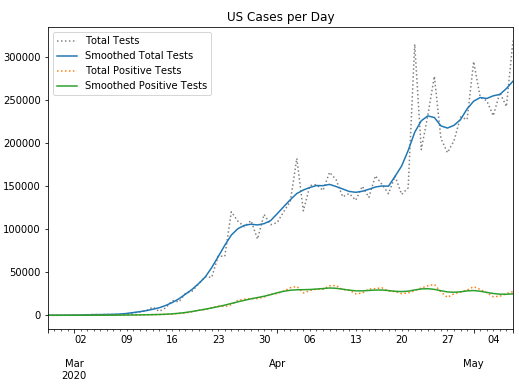
\includegraphics[width = 0.4\textwidth]{../methods/figs/US-casecount.png}
\caption{US total tests and total positive tests per day}
\label{fig:ustests}
\vspace{-0.3cm}
\end{wrapfigure}


Second, there have been calls for increased testing.  While important, many conflate increased testing capacity with increased quality of testing.  We will discuss this point further in Section \ref{section:discussion}.  As of May 8th, the US has performed $8,412,095$ tests in total.  Figure~\ref{fig:ustests} shows the trajectory of testing per day and positive cases per day in the US.  The US population is roughly $328$ million, meaning the fraction sampled is $f = 0.026$.  After smoothing, the empirical prevalence is $9.1\%$ on May 8th.  Supposing COVID-19 positive individuals are $2$ times more likely to get tested than those individuals who are COVID-19 negative, the question is ``What is the sample size from a SRS that would yield equivalent MSE in the estimated prevalence?'' Using the above MSE result, Meng showed the effective sample size is equal to $n_{eff} \leq \frac{1}{E_I [ \rho_{I,Y}^2 ]} \frac{f}{1-f}$.  Under these parameters, the effective sample size is $14$.  Recent proposals~\citep{Siddarth2020} have argued in favor of increasing overall testing capacity.  With more tests available, the relative sampling rate may reduce.  Supposing it drops to $1.2$ then the effective sample size will increase to $299$.  See Appendix~\ref{section:effss} for the mathematical details and calculations in additional scenarios.   The above calculations point to a sad state of affairs, saying that the effective sample size even in best case scenarios is not better than a small random sample from the population.

The remainder of this paper aims to build upon these fundamental insights by extending the decomposition in two directions: accounting for  measurement error and the temporal nature of the pandemic.  We then discuss effective sampling methods and their importance in the current pandemic.

\subsection{Imperfect testing}

Tests are imperfect.  COVID-19 testing is no exception. Here we investigate the interplay between imperfect testing and selection bias.  In discussions of inaccurate testing, the standard assumption is measurement error leads to parameter attenuation.  When paired with selection bias, however, the two sources of error become entangled, and resulting errors can become magnified, muted, or even switch signs.

First we require some additional notation.  Let $P_j$ be an indicator of measurement error, equal to $1$ when we incorrectly measure the outcome and $0$ when we observe the true outcome. We suppose this is a stochastic variable where $\pr(P_j = 1 \mid Y_j = 1) =: FN$ is the false-negative rate and $\pr(P_j = 1 \mid Y_j = 0) =: FP$ is the false-positive rate.  If individual $j$ is selected (i.e., $I_j = 1$) then the observed outcome can be written as $Y_j^{\star} = Y_j(1-P_j) + (1-Y_j) P_j$.  Suppose disease prevalence was estimated as the fraction who tested positive for COVID-19, i.e., $\bar y_n^\star = \frac{\sum_{i=1}^N I_j Y_j^\star}{\sum_{i=1}^N I_j}$.  We can again investigate the error compared to the true prevalence $\bar Y$ in statistical terms:
$$
\bar y_n^\star - \bar Y = \sqrt{\frac{1-f}{f}} \left[ \rho_{I,Y} \times \sigma_Y + \rho_{I,PZ} \times \sigma_{PZ} + \sqrt{\frac{f}{1-f}}  \left( FP - (FP+FN) \bar Y \right) \right] .
$$
where $Z = 1-2Y$; see Appendix~\ref{app:imperfect} for the derivation. The first term in the large brackets represents the perfect testing regime; to this end, we refer to $\rho_{I,Y}$ as the \emph{true data quality}.  The second term represents the interaction between imperfect testing and selection bias. The variable $PZ = 1[Y=0,P=1] - 1[Y=1, P=1]$ is non-zero only when $P=1$ (i.e., the outcome is incorrectly reported); to this end, we refer to $\rho_{I,PZ}$ as the \emph{observed data quality} that accounts for both selection bias and measurement error.  In the appendix, we show the sign of $\rho_{I,PZ}$ is the opposite of the sign of $\rho_{I,Y}$, which implies that the observed data quality adds error in the opposite direction from the true data quality.  Finally, the third term represents the bias due to imperfect testing.

We start by considering the first two terms and assess whether the sign of the bias can reverse due to the interaction of measurement error and selection bias.  To do this, we define the sampling rates differential.  Let $f_1 := \pr (I_J = 1 \mid Y_J = 1)$ and $f_0 := \pr(I_J = 1 \mid Y_J = 0)$ be the sampling rates.  Then $\Delta = f_1 - f_0$ is the sampling rate differential.  Using these terms, we can re-express the first two terms as
$$
\rho_{I,Y} \times \sigma_Y + \rho_{I,PZ} \times \sigma_{PZ} =
\rho_{I,Y} \times \sigma_Y \left[ 1 - \Delta \times \frac{\bar Y}{1-\bar Y} \times \frac{FP(1-\bar Y) + FN \cdot \bar Y}{f_0 (1-\bar Y) + f_1 \bar Y} \right].
$$
The final term in brackets is the \emph{measurement error adjustment to data quality} which is a complex function of sampling rate differential, the odds ratio, and the ratio of measurement error interaction with prevalence and sampling rates interaction with prevalence. Note $\sgn(\Delta) = \sgn(\rho_{I,Y})$ by equation~\ref{eq:binaryrho} in the appendix, which implies the measurement error adjustment either shrinks the data quality measure toward zero or reverses its sign.

While prior investigations have noted the interaction between measurement error and selection bias~\citep{Beesley2020,Beesley2019,Smeden2019}, the interaction with the sample size relative to the population, i.e., $f$, has largely been ignored.  The above statistical decomposition clarifies the importance of this quantity~$f$.  In particular, note that the statistical error also includes a bias term due to measurement error and this term increases as the sampled fraction $f$ increases. Therefore, how the first two terms interact with the final term depends on the fraction of the population sampled.  This interaction is complex, but implies that whether the estimate $\bar y^\star_n$ is an overestimate or underestimate is a complicated question due to the relation amongst these three pieces.

Consider again the current COVID-19 pandemic. For now, we continue to assume the ratio of conditional selection rates $f_1/f_0$ is equal to 1.5.  In Section~\ref{section:est_dq}, we discuss recent research suggesting a false negative rate around 17.2\% and a false positive rate around 0.05\%. Under these rates and the current US prevalence rates, the ratio of the MSE to MSE under no measurement error is 0.436; if we switch false negative rates down to 5\% and increase the false positive rate to 5\% then the relative MSE is 2.89.  This is merely to demonstrate that in some cases we see a huge increase in MSE and in other settings we have a huge decrease in MSE.  What drives this is the false positive and negative rate interaction with prevalence and sampling rates.  Therefore, whether we are better or worse off with respect to the MSE is a very difficult question to answer.


The attentive data analyst will recognize the estimator $\bar y_n$ is biased even for simple random samples and, if sensitivity and specificity were known a priori, may suggest the alternative estimator $\tilde y_n = \bar y_n + (1-\bar y_n) FP + FN \bar y_n$ which is unbiased under simple random sampling. We again wish to express the error $\tilde  y_n - \bar Y$ in statistical terms. In the appendix, we show that the error now can be expressed as
\begin{equation}
\label{eq:error}
\rho_{I,Y} \times \sqrt{\frac{1-f}{f}} \times \sigma_{Y}
\times \underbrace{\left[ 1 + FP + FN - \Delta \times \frac{\bar Y}{1-\bar Y} \times \frac{FP(1-\bar Y) + FN \cdot \bar Y}{f_0 (1-\bar Y) + f_1 \bar Y} \right]}_{D_M}.
\end{equation}
The first term is the same as before but increased by $(1 + FP + FN)$ to account for the additional uncertainty due to measurement error.  The second term is the interaction between selection bias and measurement error.  Figure~\ref{fig:heatmap} presents the measurement error data quality adjustment as a function of the relative frequency and odds ratio.  We see that the adjustment can be both positive and negative as well as a range of magnitudes.

We next investigate the impact of measurement error on the effective sample size calculation.  The effective sample size can now be bounded by
$$
n_{eff} \le \frac{f}{1-f} \times \frac{1}{E_{I} \left[ \rho_{I,Y}^2 D_M^2 \right]}.
$$
In Section \ref{section:est_dq}, we discuss recent studies that estimate the COVID-19 false positive rate of $0.5$\% and false negative rate $17.2$\%.  Supposing COVID-19 positive individuals are $2$ times more likely to get tested than those individuals who are COVID-19 negative, the effective sample size drops from $14$ to $10$. If the relative sampling fraction drops to $1.2$ then the effective sample size drops from $299$ to $216$.

\begin{wrapfigure}{r}{0.5\textwidth}
\centering
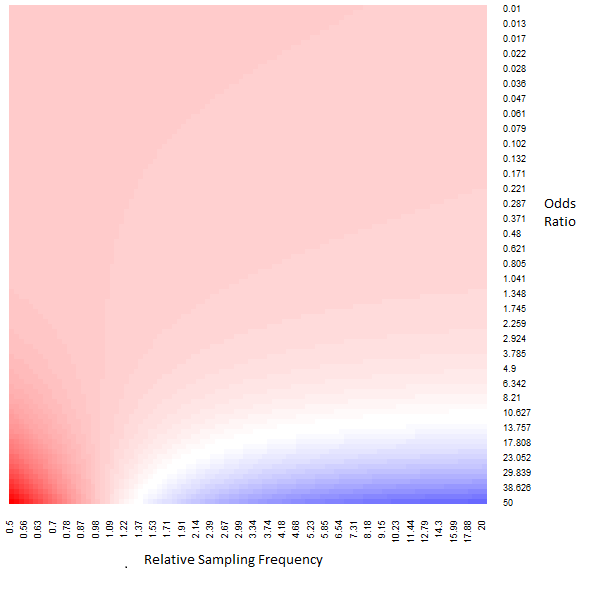
\includegraphics[width = 0.4\textwidth]{../methods/figs/mem_heatmap_article.png}
\caption{Measurement error data quality adjustment: relative frequency $f_1/f_0$ (x-axis) against odds ratio (y-axis) for $FP=0.005$ and $FN=0.172$. Color scaled so blue = $-10$, white = $0$, and red = $10$.}
\label{fig:heatmap}
\vspace{-0.3cm}
\end{wrapfigure}


The above argument shows that the effective sample size is affected in a complex manner by the interaction between selection bias and measurement error.  Here, we discuss the impact of the interaction on the effective sample size when testing capacity is tied to measurement error.  In the current COVID-19 pandemic, there have been well-justified calls for increases in testing capacity.  These increases, however, may come at the cost of increases in false-positive and false-negative rates.  In terms of effective sample size, if the data quality term remains constant, then testing increases may not significantly improve the effective sample size.  Consider the simplest case where $f$ increases from $0.05$ to $0.1$; suppose this increase was associated with  false positive rate increasing from $0.5$\% to $5$\% and the false negative rate rising from $5\%$ to $20$\%.  Then the standard analysis would suggest a reduction in the MSE by 47\% but the actual decrease is by 26\%.  This implies that doubling the sampling rate will only increase the effective sample size by a factor $2.9$ rather than the expected $4$ fold increase that is expected.  In a worst case scenario, if the false negative rate climbs to $0.30$ and the false positive rate to $0.10$ then the factor effective sample size increases by only a factor of $2.3$.

\subsection{Regrettable rates: complex biases resulting from self-selection}
\label{section:rates}

The data analyst, now wary of estimating prevalence and total counts, pauses and thinks.  They return shortly thereafter, with a follow-up consideration: \emph{Ok, perhaps estimating prevalence is difficult. Certainly, however, we can estimate the rate of growth.  All I want to know is when we hit the point at which the curve flattens and number of deaths decrease.  That can't be too hard, surely!}

Unfortunately, ratio estimators do not cancel errors as now both the numerator and the denominator are uncertain.  This means selection bias and measurement error can have paradoxical effects.  Here we consider the ratio estimators for the relative change in the prevalence rate.  We let $\bar Y_{t-1}$ and $\bar Y_{t}$ denotes the prevalence (across the entire population) at time step $t-1$ and $t$ respectively (i.e., prevalence on two consecutive days).  Then the ratio estimator is given by $r = \bar y_t / \bar y_{t-1}$.  We assume both numerator and denominator are the prevalence estimates adjusted for measurement error. If the sample size at each time were equal (i.e., $n_1 = n_2 = n$) then this analysis would be equivalent to comparing the increase in observed case-counts (i.e., $\bar y_t/\bar y_{t-1} = y_t/y_{t-1}$).  We wish to express the error $\frac{\bar y_t}{\bar y_{t-1}} - \frac{\bar Y_{t}}{\bar Y_{t-1}}$ in statistical terms.  Using a Taylor series approximation, we show in the appendix that the error can be expressed approximately as
$$
\begin{aligned}
\frac{\bar Y_t}{\bar Y_{t-1}} &\times \bigg[ \rho_{I_t,Y_t} D_{M_t} \sqrt{\frac{1-f_t}{f_t}} CV (Y_t)  -\rho_{I_{t-1},Y_{t-1}} D_{M_{t-1}} \sqrt{\frac{1-f_{t-1}}{f_{t-1}}} CV (Y_{t-1}) \bigg] \\
&\times \left[ 1 - \rho_{I_{t-1},Y_{t-1}} D_{M_{t-1}} \sqrt{\frac{1-f_{t-1}}{f_{t-1}}} CV (Y_{t-1}) \right]
\end{aligned}
$$
where $\rho_{I_j, Y_j}$ is the data quality, $f_j$ is the sampling fraction, $D_{M_j}$ is the measurement error adjustment, and $CV(Y_j) = \sigma_{Y_j}/\bar Y_j$ is the coefficient of variation at time step $j$.  The magnitude of the error depends on the population-level ratio $\bar Y_{t} / \bar Y_{t-1}$ so a large decrease in the prevalence rate will have a relatively small error as compared to a large increase in the prevalence rate. The second term represents the ``cancellation'' that the naive analyst is hoping will occur.  The analyst's intuition only holds when the difference is equal to zero.  This occurs at times when data quality, sampling fraction, measurement error, and prevalence are all constant across time.

Consider the state of New York.  Figure~\ref{fig:ny-covid-test} shows the number of tests and positive tests per day in New York state.  Figure~\ref{fig:ny-covid-frac} presents the fraction of tests that were positive per day in New York state.  For cancellation, we would need the expected data qualities to be uncorrelated and equal. Testing appears relatively stable over a week which suggests assuming $\Delta_t$ (i.e., differential in the selection rate) varies slowly over time may be a plausible assumption.  Note, however, that constant $\Delta_t$ does not imply constant data quality (see Appendix \ref{section:effss} for details).  Figure~\ref{fig:ny-covid-test} shows the number of tests has remained relatively constant in the last few weeks, specifically relative to the total NY population, assuming $f_t$ also varies slowly in time is reasonable. Finally, the measurement error adjustment is likely to be constant as no new testing procedures have been reported.  This would not be true in states like Michigan, where testing criteria have been expanding every few weeks.  The final component is an adjustment to this differential error based on the statistical error at the first time point.


Figure \ref{fig:ratio-bias} shows a trajectory of the true ratio and the potential biased estimators under an SIR model for the epidemic dynamics, with state evolution given by the following ODE
$$
\begin{aligned}
\frac{\partial S_t}{\partial t} &= - \beta S_t I_t N^{-1}; \quad
\frac{\partial I_t}{\partial t} = \beta S_t I_t N^{-1} - \gamma I_t; \quad
\frac{\partial R_t}{\partial t} = - \gamma I_t \\
\end{aligned}
$$
where $S_t$ is the number of susceptible individuals at time $t$, $I_t$ is the number of infected individuals at time $t$, $N$ is the total population size, and $R_t$ is the number of removed (recovered or deceased) individuals at time $t$.   Figure~\ref{fig:fracpop} presents the fraction of population newly infected individuals at each time step for $\beta = 1.4$ and $\gamma = 0.2$ (black line).  In each case, the rate of change in prevalence is likely to be  overestimated prior to the peak and then underestimated afterwards.  From a decision making perspective, such biases have potential impact.  First, the over-estimation may give lawmakers and governors more leverage in proposing aggressive actions that reduce prevalence.  Of course, the analysis supports the argument that the estimates based on available data are overly pessimistic. What both sides miss is that the direction of bias is non-constant over time.  After we hit the peak, estimates will likely under-estimate prevalence.  Such bias puts pressure on lawmakers and governors to prematurely relax social distancing measures.  Moreover, the question is ``Can we trust the observed data to let us know if we have reached the peak?''  It appears that the peak time is the easiest to estimate in terms of having minimal error using availability data.  Note, however, that the standard errors on such estimates will be incredibly wide due to the low effective sample size as discussed in Section~\ref{section:casecount}.

\subsection{Estimation of effective reproduction number}
\label{section:r0-estimation}
Many well-respected epidemiologists argue that tracking the effective reproduction number $R_t$ is the only way to manage through the crisis~\citep{Gabriel2020}.  We show here how these estimates are also impacted by selection bias and measurement error.  For simplicity, we again assume the estimates are adjusted for known false positive and false negative rates. \cite{Bettencourt2008} show that under a Poisson likelihood, a simple relation between the trajectory of new cases and the effective reproduction number can be derived.  In particular, under an SIR model, the number of case counts on day $t$ is Poisson distributed with rate $K_{t-1} \exp \left( \frac{1}{\gamma} (R_t - 1) \right)$ where $K_{t-1} = Y_{t-1}-Y_{t-2}$ is the number of new cases on day $t-1$ and $\gamma$ is the serial interval which is approximately $7$ days for COVID-19~\citep{Sanche2020}.  Using this, a simple estimator of the effective reproduction number at time $t$ can be given by
$$
R_t = 1 + \frac{1}{\gamma} \log \left( \frac{K_t}{K_{t-1}} \right).
$$
Of course, we do not observe $K_t$ and $K_{t-1}$ but noisy proxies $y_t$ and $y_{t-1}$, i.e., the observed case-count on day $t$ and $t-1$ respectively. The hope is that $y_t/y_{t-1}$ is a good proxy for $K_t/K_{t-1}$ where here $y_t$ is conceptualized as the number of new cases on day $t$. However, if we think about estimating number $K_t$ under SRS of new cases among those susceptible on day $t$, the natural estimator is $S_t \bar y_t$.  Unfortunately the number of individuals susceptible on day $t$ is unknown.  Here, we assume that $\hat R_t = 1 + \frac{1}{\gamma} \log \left( \bar y_t / \bar y_{t-1} \right)$ is the estimated effective reproduction number on day $t$.
This estimator adjusts for sample size variation across days but not the varying population size. The estimator is close in spirit to the estimator derived under assuming the process is fully observed.  Similar to Section~\ref{section:rates}, the proxy has error in both numerator and denominator that may cause issues.  We again wish to express the statistical error of $\hat R_t - R_t$ in useful terms.  We can re-arrange the error decomposition from Section~\ref{section:rates} to show that this error is given by
$$
\begin{aligned}
\frac{1}{\gamma}\log &\bigg( 1 + \bigg[ \rho_{I_t,K_t} D_{M_t} \sqrt{\frac{1-f_t}{f_t}} CV (K_t)  -\rho_{I_{t-1},K_{t-1}} D_{M_{t-1}} \sqrt{\frac{1-f_{t-1}}{f_{t-1}}} CV (K_{t-1}) \bigg] \\
&\times \left[ 1 - \rho_{I_{t-1},K_{t-1}} D_{M_{t-1}} \sqrt{\frac{1-f_{t-1}}{f_{t-1}}} CV (K_{t-1}) \right] \bigg) - \frac{1}{\gamma} \log \left( \frac{S_t}{S_{t-1}} \right).
\end{aligned}
$$
So here we see the exact same trade-off as with the rates but on the logarithmic scale.  For small values of $x$, we have $\log(1+x) = x$ and so the biases are similar.  However, the error is no longer scaled by the rate of change in prevalence $\bar Y_2/\bar Y_1$. Instead the error is scaled by the serial interval $\gamma^{-1} = 1/7$.  Moreover, the error depends not on aggregate prevalence $\bar Y_t$ but fraction of new cases $\bar K_t$. The final term is the error due to varying population sizes.  Since $S_t \leq S_{t-1}$, the final term $- \log (S_t/S_{t-1}) \geq 0$. Figure~\ref{fig:r0-bias} displays the bias for the effective reproductive number and how it is impacted by the relative sampling fraction.  Here for simplicity, we assume the fraction of the population that is susceptible remains large and near the total population size.  Under these assumption, the potential bias is similar to that for the ratio estimator adjusted to be on the logarithm scale.  Changes to this assumption can impact the potential bias.  The key difference between Figure~\ref{fig:ratio-bias} and Figure~\ref{fig:r0-bias} is that prevalence depends on the fraction of the population infected at time $t$ while $\hat R_t$ depends on the fraction of new cases in the population. This leads to differences in when the bias is most pronounced.

\begin{figure}
\centering
\begin{subfigure}{.5\textwidth}
  \centering
  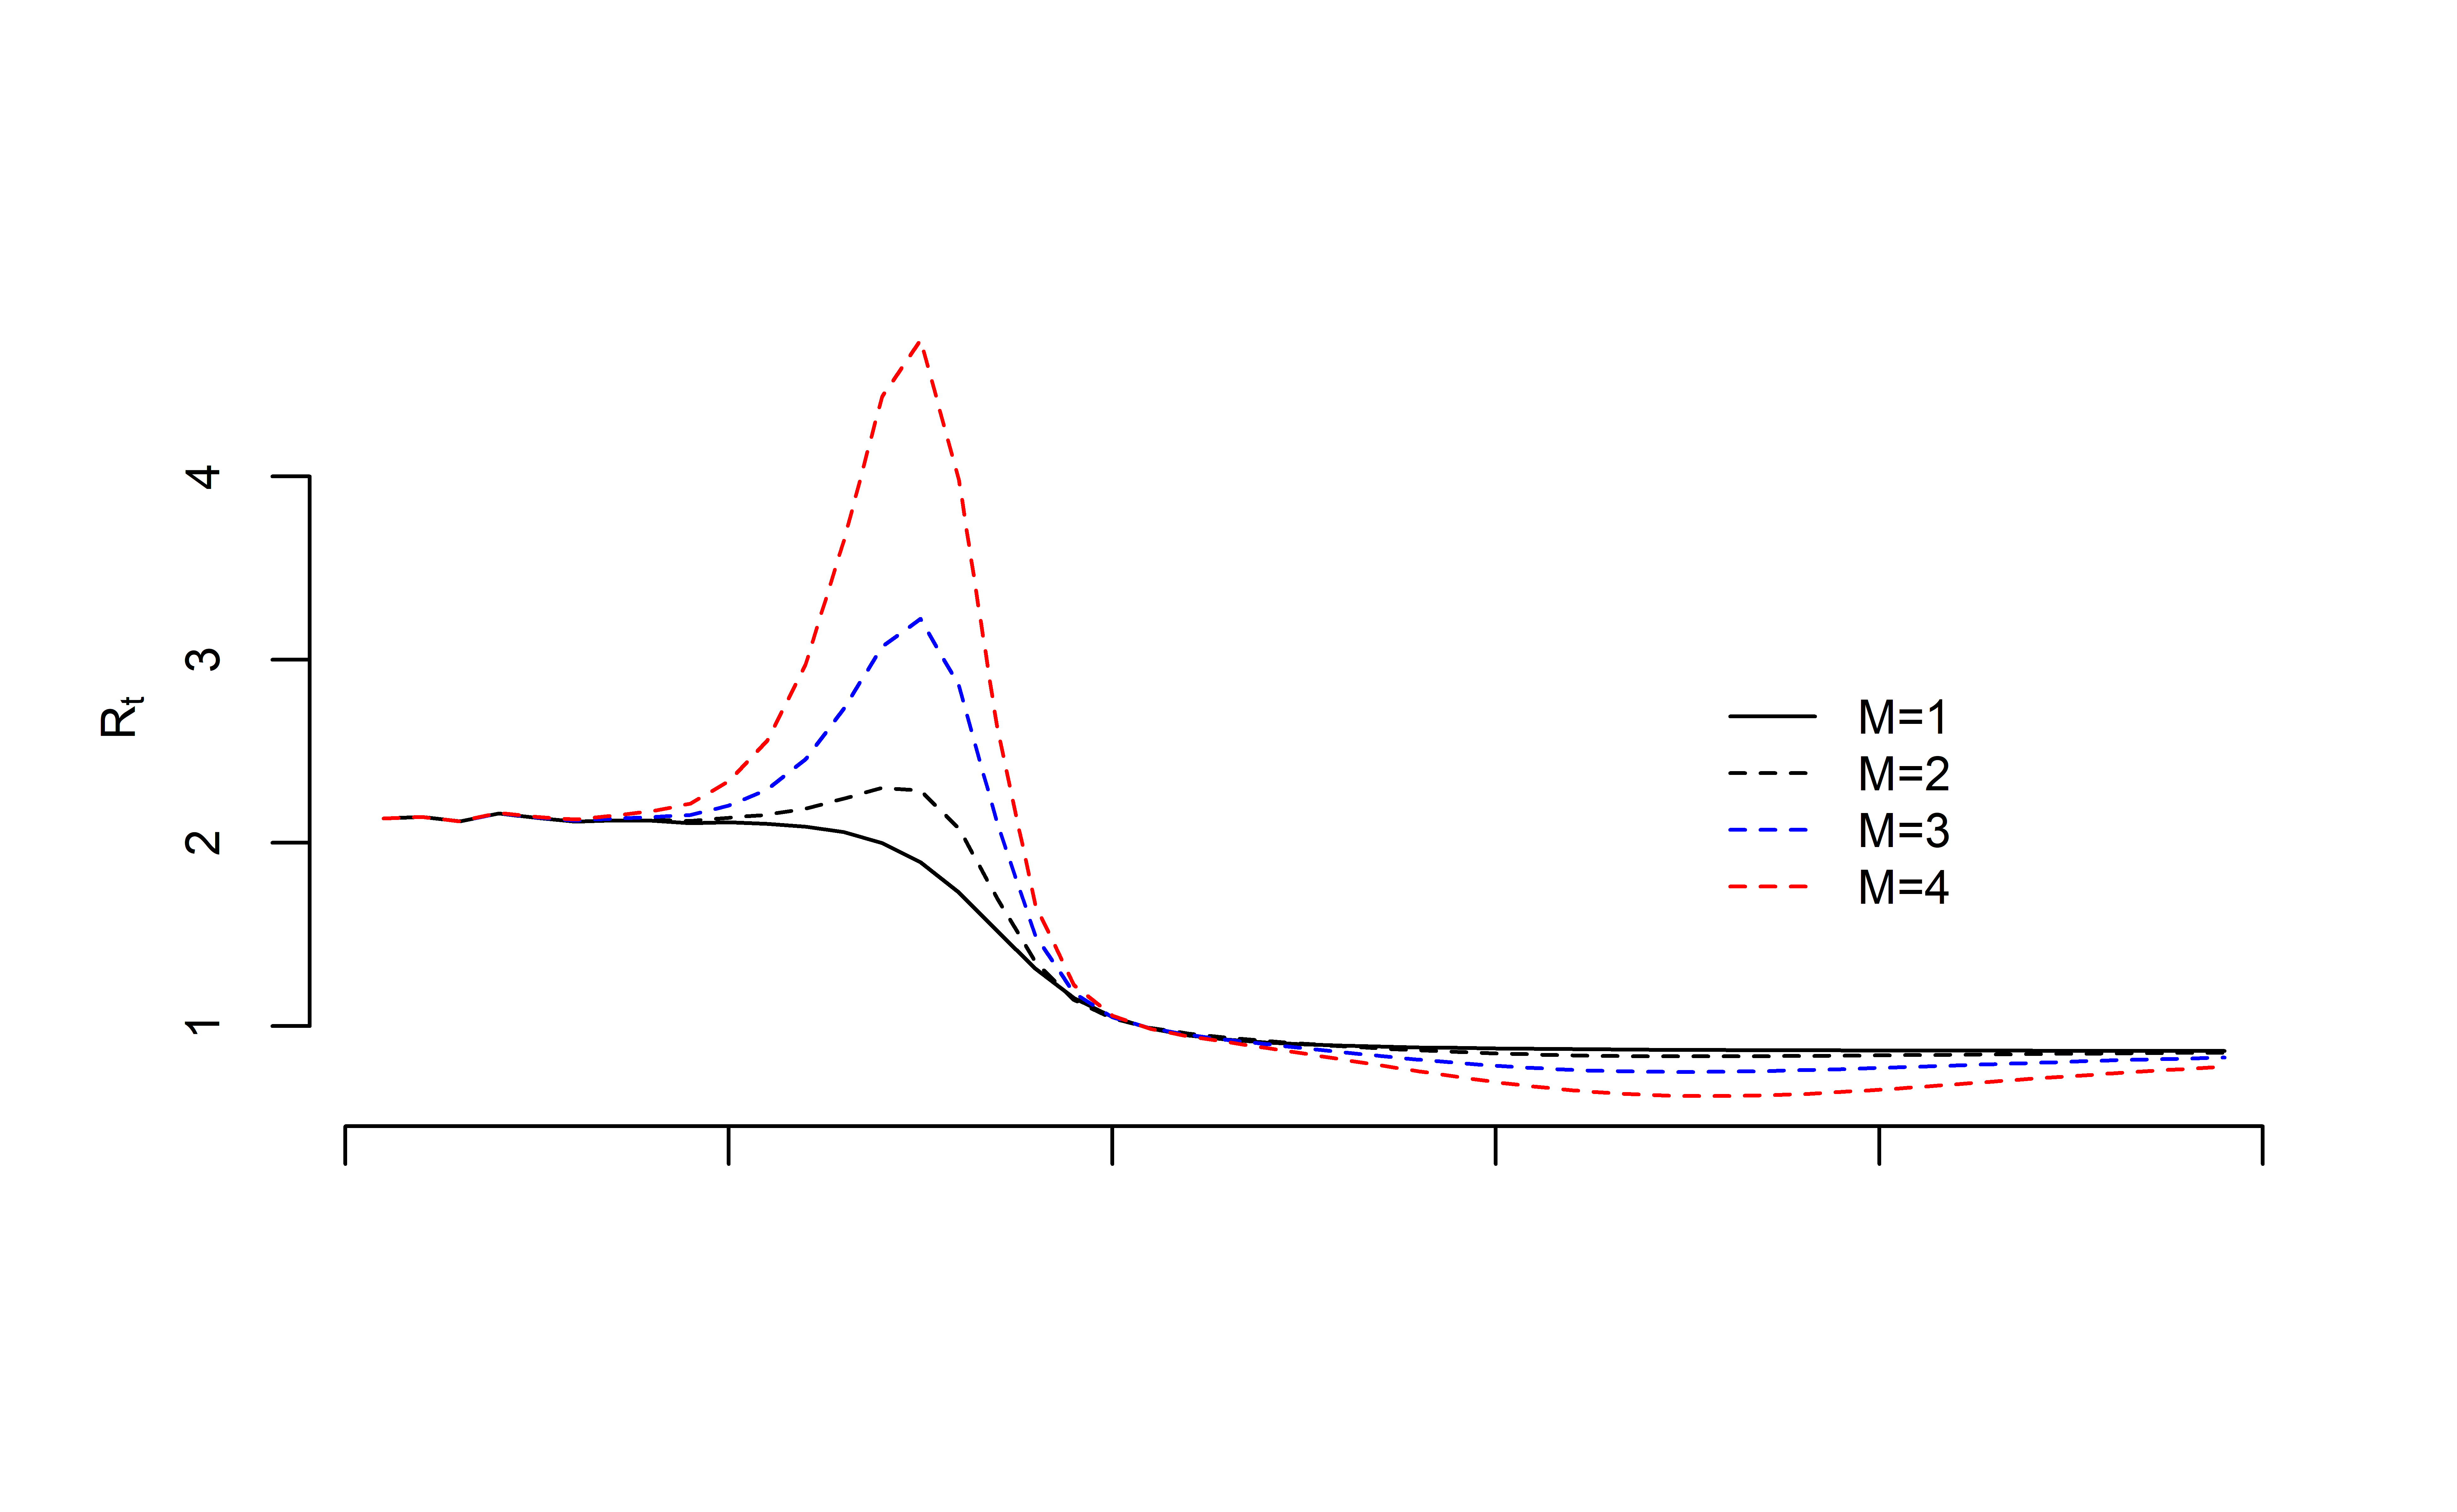
\includegraphics[width=.9\linewidth]{../methods/figs/sir_ratio.png}
  \caption{Ratio estimator}
  \label{fig:ratio-bias}
\end{subfigure}%
\begin{subfigure}{.5\textwidth}
  \centering
  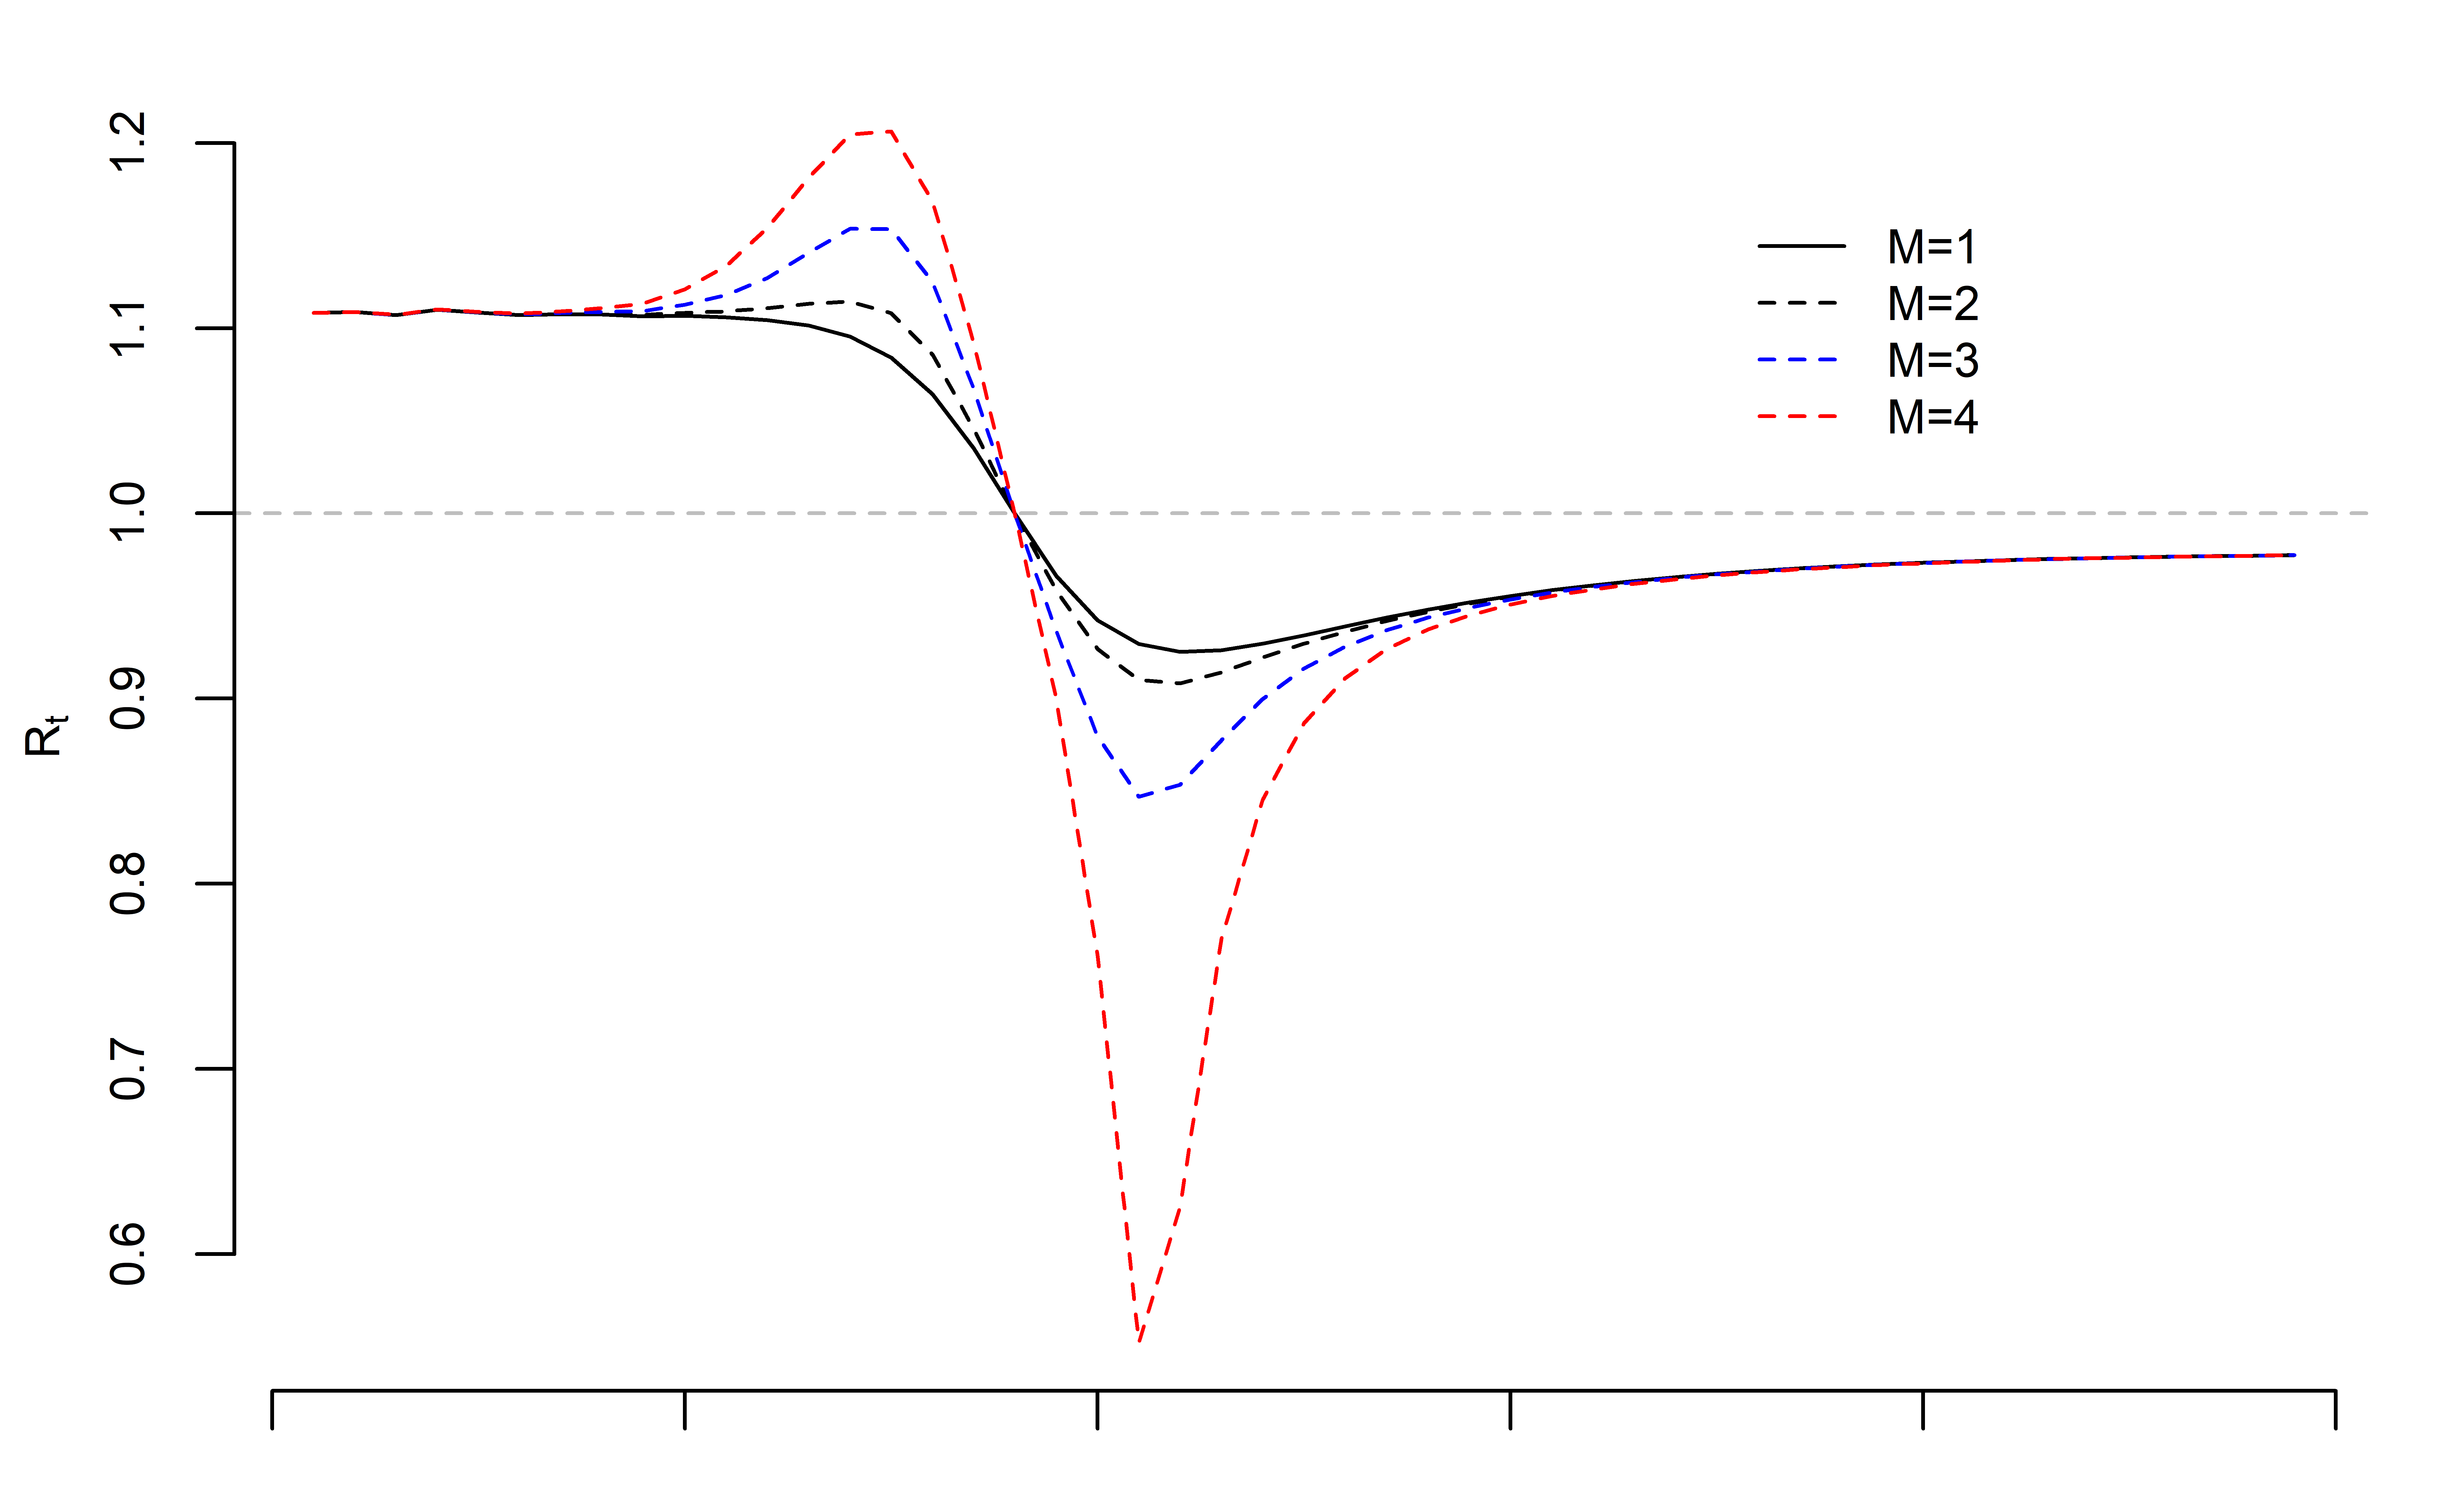
\includegraphics[width=.9\linewidth]{../methods/figs/sir_rt.png}
  \caption{Effective reproductive rate estimator}
  \label{fig:r0-bias}
\end{subfigure}
\caption{Potential bias due to self-selection and measurement error from a deterministic SIR model with $\beta = 1.4$ (black) and $\gamma = 0.2$ (red).  Here we assume $f = 0.02$, $FP = 0.01$, $FN = 0.15$, and use a range of relative sampling fraction $M = f_1/f_0$.}
\label{fig:rates}
\end{figure}

\subsection{Effect modifiers in COVID-19 clinical trials}

Here we show how selection bias and measurement error can creep into clinical trial analysis. The key concern is whether clinical trials on COVID-19 recruit from the pool of individuals who have tested positive for COVID-19 or whether they sample randomly from the population, test, and then recruit from this subset of tested individuals.  To see this issue, suppose we have an outcome $Y$, a treatment $A$ and an \emph{unobserved} variable $U$.  Suppose treatment is assigned at random, i.e., $A =1$ with probability $50\%$ and $A=0$ with probability $50\%$.  Suppose the conditional mean of the outcome satisfies  $E(Y \mid U, A ) = \beta_0 + \beta_1 A + \beta_2 U + \beta_3 A U$.  Typically, we are interested in the \emph{causal effect} of $A$ on $Y$.  In counterfactual language,
$$
E( Y(A=1) - Y(A=0) ) = E_U ( E_A ( Y(A=1) - Y(A=0) \mid U=u ))
= \beta_1 + \beta_3 E(U).
$$
Even in a randomized experiment, the question is what the correct value for $E(U)$ is. For COVID-19, the value of interest is the expected value of $U$ in the population of COVID-19 positive individuals.  Due to selection bias, however, the bias in this marginal treatment effect compared to the true marginal effect of interest is $\beta_1 \cdot E_{\I} [ \rho_{I,U} ] \times \sqrt{ \frac{f}{1-f} } \times \sigma_U$.  Selection bias then leads to the estimated effect being biased if $\beta_1 \neq 0$.  Directionality of the bias will depend on the relationship between $U$ and $Y$.  If $U$ is a measure of disease severity, then it could be expected to see $\beta_1 > 0$ and $E_{\I} [ \rho_{I, U} ] >0$.  In such situations, the treatment effect estimates will tend to be overly optimistic as most individuals recruited are potentially higher on the severity index than the population average.  Not only that, but for fixed data quality, the error compared to SRS in terms of effect estimation scales with the population size (i.e., the law of large populations).

Randomization of treatment assignment in clinical trials negates unobserved confounders.  This, however, does not negate effect modifiers.  Therefore, for marginal treatment effects to be interpretable, there must be a well-defined population.  Most often, our main interest is in causal effects on the population of COVID-19 positive.  Randomization within the clinical trial design yields internal validity, but we also need external validity to estimate the correct marginal effect of interest.

\section{Cross-population comparisons}

So far we have focused on understanding the limitations of using case-count data to understand population quantities of interest for a \emph{single} population (i.e., United States, Germany, France or Michigan, New York, London in isolation) at a single moment and over time.  Many are interested in cross-population comparisons.  Many pieces in the media as well as academic articles have plots of case-count over time aligned by time of first known case.  Others have claimed such comparisons unfair due to unequal population sizes and instead plotted case-count per million.  In this section, we focus on the statistical issues relevant to such comparisons. We do not make any comments on the multi-causal nature of success/failure in countries.

\subsection{Prevalence comparisons}

At a fixed time, suppose prevalence estimates $\bar y_1$ and $\bar y_2$ are observed for two populations. We can express $\bar y_1 - \bar y_2$ in statistical terms as
$$
(\bar Y_1 - \bar Y_2) + \left[ \rho_{I_1, Y_1} \times D_{M_1} \times \sqrt{\frac{1-f_1}{f_1}} \times \sigma_{Y_1}  - \rho_{I_2, Y_2} \times D_{M_2} \times \sqrt{\frac{1-f_2}{f_2}} \times \sigma_{Y_2} \right].
$$
The first term is the difference in population prevalence (i.e., the quantity of interest).  If random sampling were performed in each population, $E_{\I} [ \rho_{I_j, Y_j}] = 0$ and so the estimate would be unbiased.  However, the second term represents the complex error that results from selection bias.
The particular test of interest is $H_0: \bar Y_1 = \bar Y_2$.  Under the null, $\sigma_{Y_1} = \sigma_{Y_2}$.  In classical statistics, we would compute a Z-score:
$$
\begin{aligned}
\frac{\bar y_1 - \bar y_2}{ \sqrt{V_{SRS} (\bar y_1 - \bar y_2)} } &=
\frac{\rho_{I_1, Y_1} \times D_{M_1} \times \sqrt{\frac{1-f_1}{f_1}}  - \rho_{I_2, Y_2} \times D_{M_2} \times \sqrt{\frac{1-f_2}{f_2}} }{ \sqrt{\frac{1}{N_1 -1} \times \frac{1-f_1}{f_1} + \frac{1}{N_2 - 1} \times \frac{1-f_2}{f_2}} }  \\
&\overset{\star}{=}
\sqrt{\frac{(N_1-1)(N_2 -1)}{N_1 + N_2}} \left[ \rho_{I_1, Y_1} - \rho_{I_2, Y_2} \right]
\end{aligned}
$$
Where the last equality holds under $f_1 = f_2$, i.e., same sampling rate relative to population size. This tells us that the exact error in the comparison of sample means, as an estimate of the difference in population means, scales as a function of the difference in data quality $\rho_{I_1, Y_1} - \rho_{I_2, Y_2}$ times a square root of a population adjustment.  For highly unequal population sizes (e.g., $N_1 \gg N_2$), the adjustment is approximated well by the square root of the smaller population size minus one (e.g. $\sqrt{N_2 -1}$).

Take, for example, a comparison of the US and Canada.  The two population sizes are approximately 328 million and 38 million people.  Then the population adjustment is $5.84$ million. As of May 5th, Canada has performed a total of 24.92 tests per 1,000 people while the US has performed a total of 22.01 tests per 1,000 people\footnote{According to \href{https://ourworldindata.org/grapher/full-list-cumulative-total-tests-per-thousand}{ourworldindata.org}} so the data quantities are approximately equal to $f = 23/1000 = 0.023$.  Then, under a prevalence of 10\%, one would need the differential $\Delta_1-\Delta_2$ to be much smaller than $11.68 \times 10^{-6}$ in order for the selection bias to not impact.  So only under the very strong assumptions of equal data quantity and quality will the comparisons be valid and the $Z$-score can be treated as in the classical setting.  A simple alternative is to use the effective sample sizes to build more appropriate $Z$-score.  That is, setting
$$
Z_n = \frac{\bar y_1 - \bar y_2}{ \frac{1-f}{f} \sigma_y \sqrt{ \frac{1}{n_{1,eff} - 1} + \frac{1}{n_{2,eff} - 1}}}
$$
allows us to build Z-scores that account for the true sample size.  While still not perfect, this allows us to build Z-scores that are not overly confident due to selection bias and measurement error.  See Section~\ref{section:est_dq} for discussion of how to estimate data quality.

\subsection{Case count comparisons}
Two alternative comparisons are common. First, the data analyst may directly compare the observed number of new cases on a given day.  If $Y_1$ and $Y_2$ are the number of cases in locations $j=1,2$ respectively, then we can express the error of $y_1 - y_2$ as
$$
\begin{aligned}
y_1 - y_2 &= n_1 ( \bar y_1 - \bar Y_{1}) - n_2 ( \bar y_2 - \bar Y_{2}) + \left( \frac{n_1}{N_1} Y_{1} - \frac{n_2}{N_2} Y_2  \right) \\
&= \left[ n_1 \sigma_{Y_1} \rho_{I_1, Y_1} \sqrt{\frac{1-f_1}{f_1}} D_{M_1} - n_2 \sigma_{Y_2} \rho_{I_2, Y_2} \sqrt{\frac{1-f_2}{f_2}} D_{M_2}  \right] + \left[ f_1 Y_1 - f_2 Y_2 \right].
\end{aligned}
$$
Under simple random sampling, the first term is zero in expectation.  However, the question is whether $f_1 \bar Y_1 - f_2 \bar Y_2$ is of scientific interest.  We would argue that this is only of true interest when $f_1 = f_2$ and we are interested in comparing total number of cases.  In this setting, however, the difference in error terms is unlikely to be zero.  To see this, assume that we have similar expected data quality, data quantity, problem difficulty, and measurement error.  Then the error is a function of $n_1 - n_2 = n_2 \left( \frac{N_1}{N_2} - 1 \right)$.  So we see that the error now is a function of the relative difference in the population sizes.

Alternatively, the data analyst may be wary of such concerns in population differences and scale counts by respective population size, i.e., $y_1/N_1 - y_2/ N_2$.  We can again express the error as
$$
\begin{aligned}
\frac{y_1}{N_1} - \frac{y_2}{N_2} &= \frac{n_1}{N_1} ( \bar y_1 - \bar Y_{1}) - \frac{n_2}{N_2} ( \bar y_2 - \bar Y_{2}) + \left( \frac{n_1}{N_1} \bar Y_{1} - \frac{n_2}{N_2} \bar Y_2  \right) \\
&= \left[ \sigma_{Y_1} \rho_{I_1, Y_1} \sqrt{ f_1 (1-f_1) } D_{M_1} - \sigma_{Y_2} \rho_{I_2, Y_2} \sqrt{f_2 (1-f_2)} D_{M_2} \right] + \left[ f_1 \bar Y_1 - f_2 \bar Y_2 \right].
\end{aligned}
$$
Under simple random sampling, the first term is again zero in expectation.  However, the question is whether $f_1 \bar Y_1 - f_2 \bar Y_2$ is of scientific interest.  We would argue that this is only of true interest when $f_1 = f_2$ and we wish to compare disease prevalence.  Importantly, the error in this comparison is less problematic.   To see this, assume that we have similar expected data quality, data quantity, problem difficulty, and measurement error.  Then the error is equal to zero.

It is important to note that the standard law of large populations caveats apply to both comparisons.  In both cases, the point is that we must ascertain what is the population-level contrast and whether this should be of genuine scientific interest. Otherwise, we are comparing apples and oranges.  Not only this, but the two comparisons come with different levels of error induced by selection bias and measurement error.

\subsection{Rate comparisons}

An alternative is the comparison on the rates of case-count change over time.  Here, for simplicity, we focus on comparing the estimated effective reproductive rate.  We assume the two time-series are aligned so that $t=0$ is the time of first case.  This negates alignment issues and is common in practice.

While the above issues on $Z$-scores and effective sample size are important, here we highlight a separate issue.  Namely, the interaction of biases in estimation of the two trajectories when the peak infection times differ slightly.  We can write the difference in the rates as
$$
R_{t1} - R_{t2} = \frac{1}{\gamma} \log \left( \frac{1 + e_{1t}}{1+e_{2t}} \right)
$$
where $e_{jt}$ is the error associated given in Section \ref{section:r0-estimation}.  Recall that the error allowed for over-estimation prior to the peak and then under-estimation post-peak.  Here, these errors can mingle in interesting ways.  Consider two countries (A and B) in which the peak occurs 2 weeks prior for country A then country B but other.  Figure~\ref{fig:comparison} presents such a comparison where each country's disease trajectory follows an SIR model as described in Section~\ref{section:rates} with different parameters.  Figure \ref{fig:eff} shows how the errors interact in complex ways.  First, the gap is correctly estimated; then the gap is over-estimated as country A sees a rapid rise in cases; then the gap is even more over-estimated as country A improves and the rate is under-estimated while country B sees a rapid increase in their case-count and their rate is over-estimated; then country A's rate is correctly estimated while country B's rate is under-estimated as it sees improvement in infection rates; finally, the gap disappears.  We are not claiming this will always be the case, and indeed for small enough selection bias and/or large gaps in case-counts such complex behaviour will not occur; however, this is simply to point out how observed information can tell a more complex story than the truth (i.e., country A recovers 1 month prior to country B).

\begin{figure}
\centering
\begin{subfigure}{.5\textwidth}
  \centering
  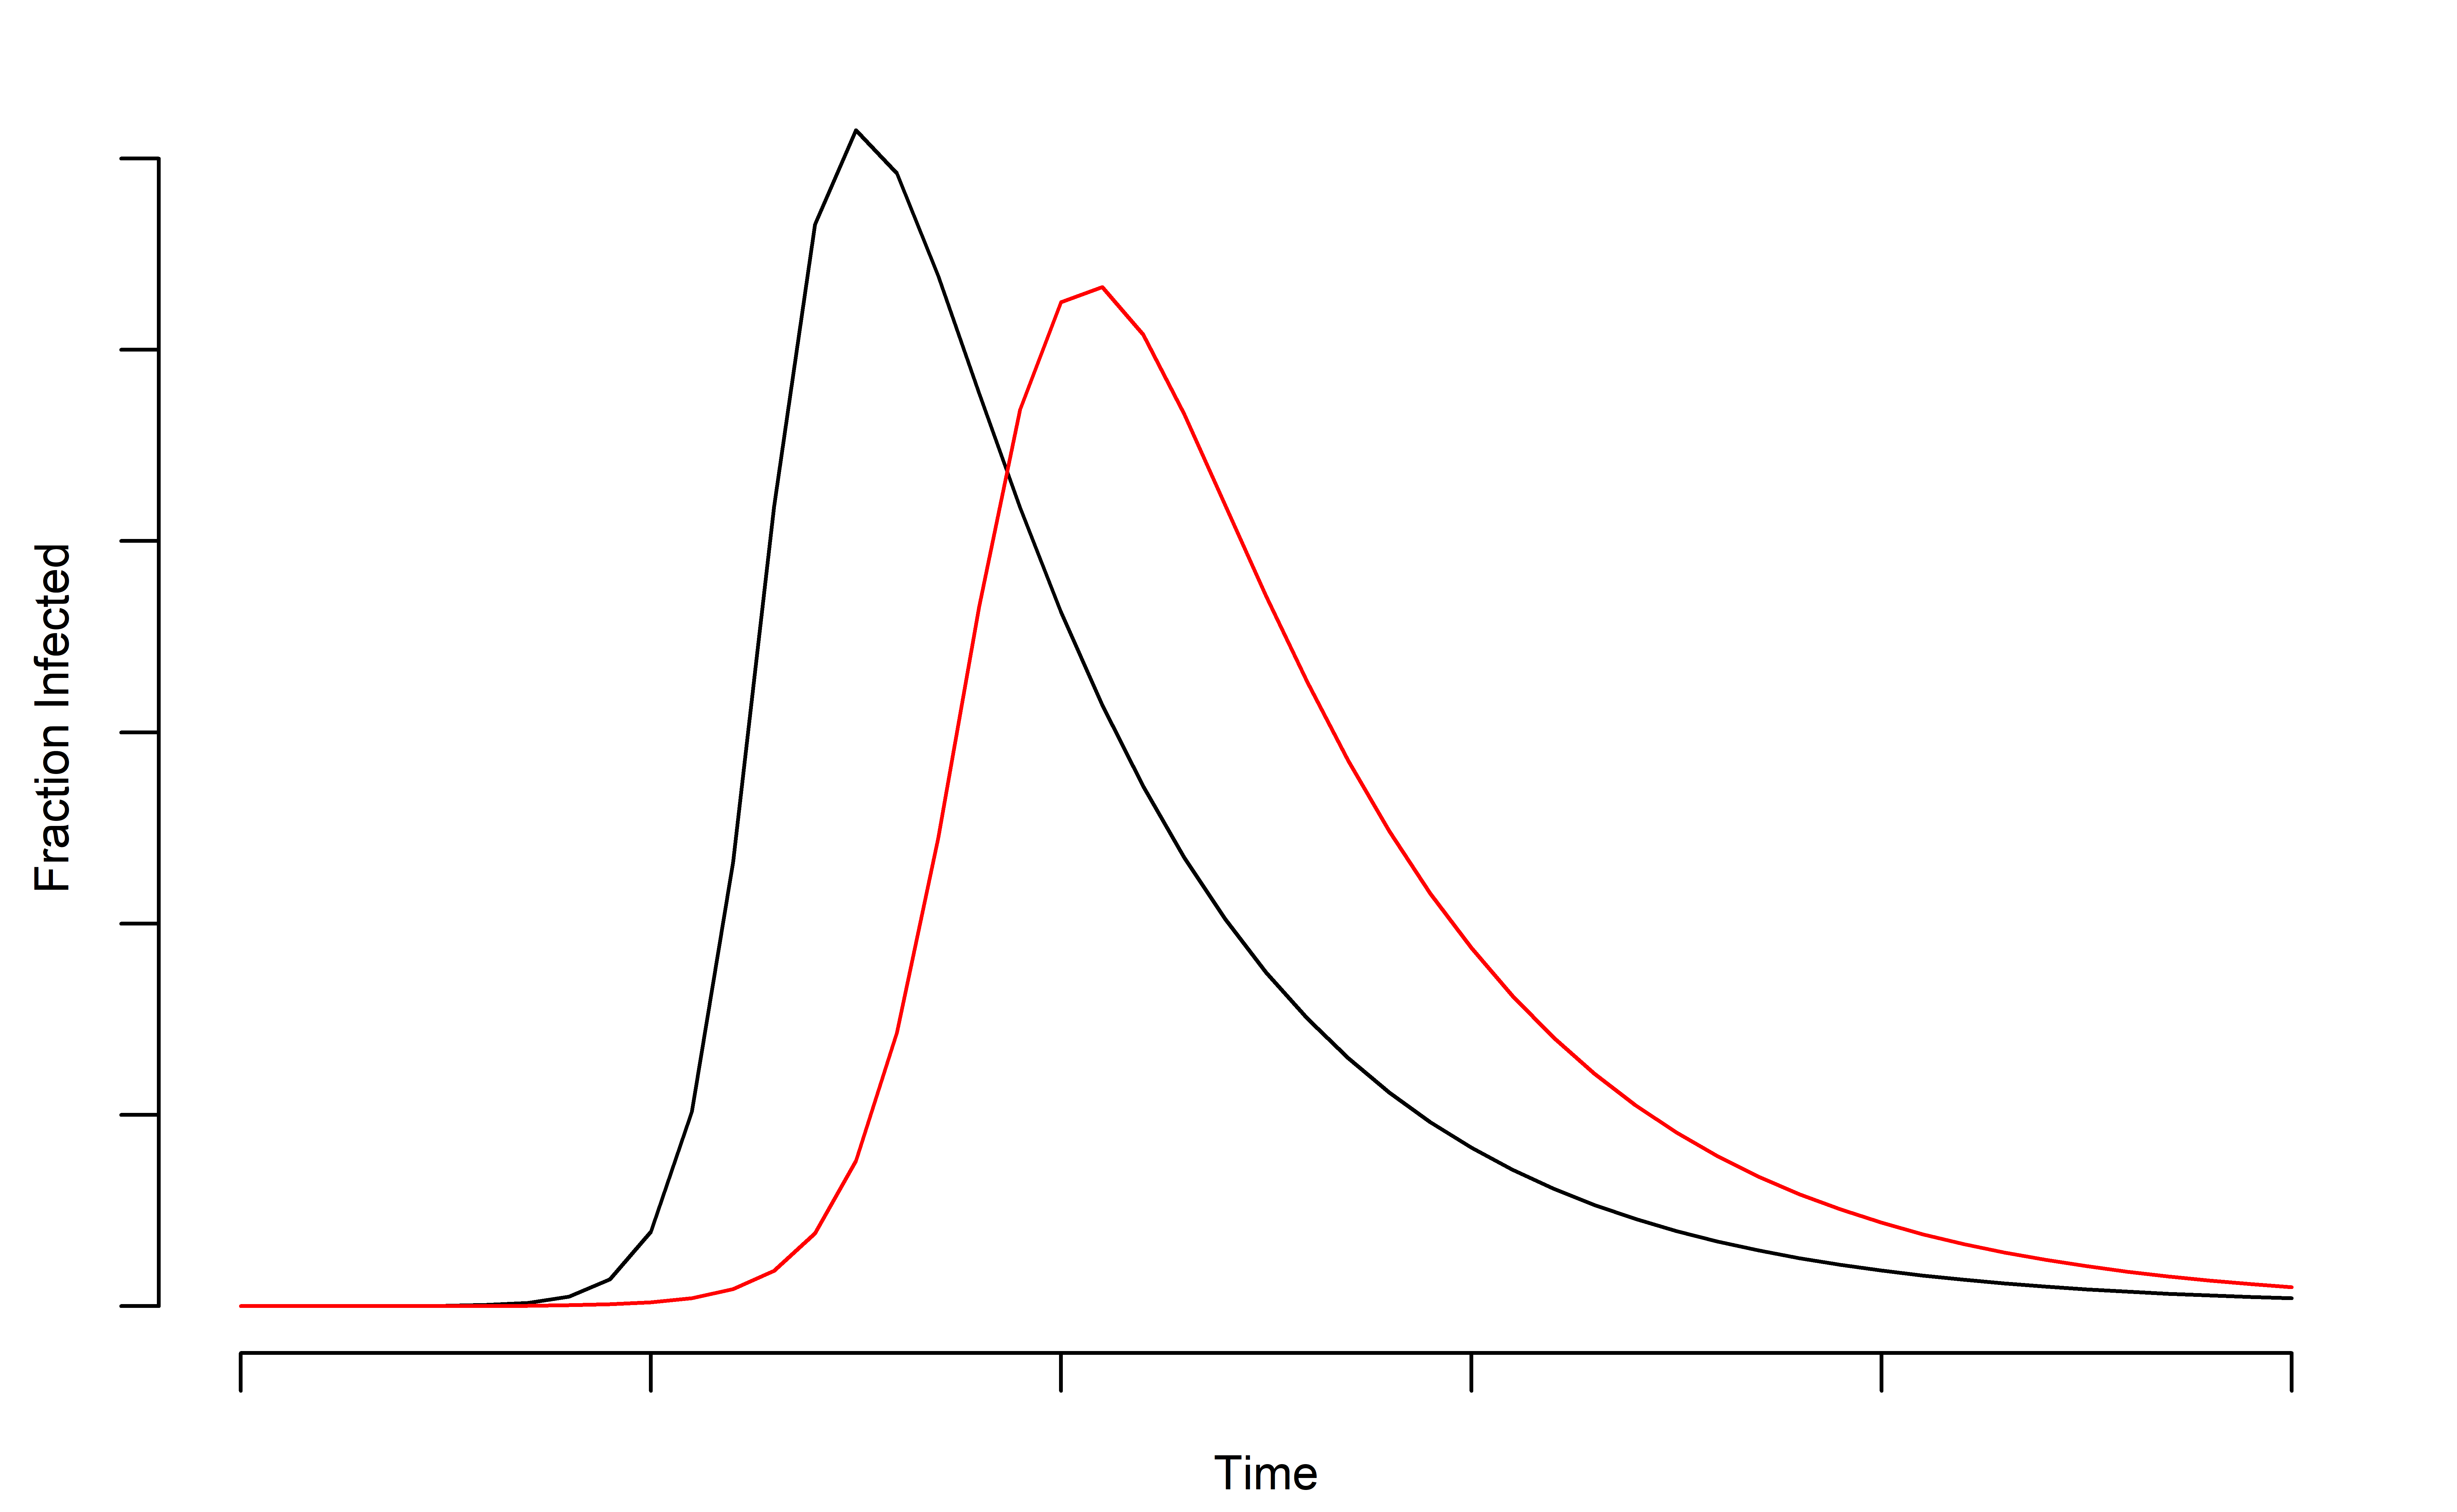
\includegraphics[width=.9\linewidth]{../methods/figs/sir.png}
  \caption{Fraction of new cases in population}
  \label{fig:fracpop}
\end{subfigure}%
\begin{subfigure}{.5\textwidth}
  \centering
  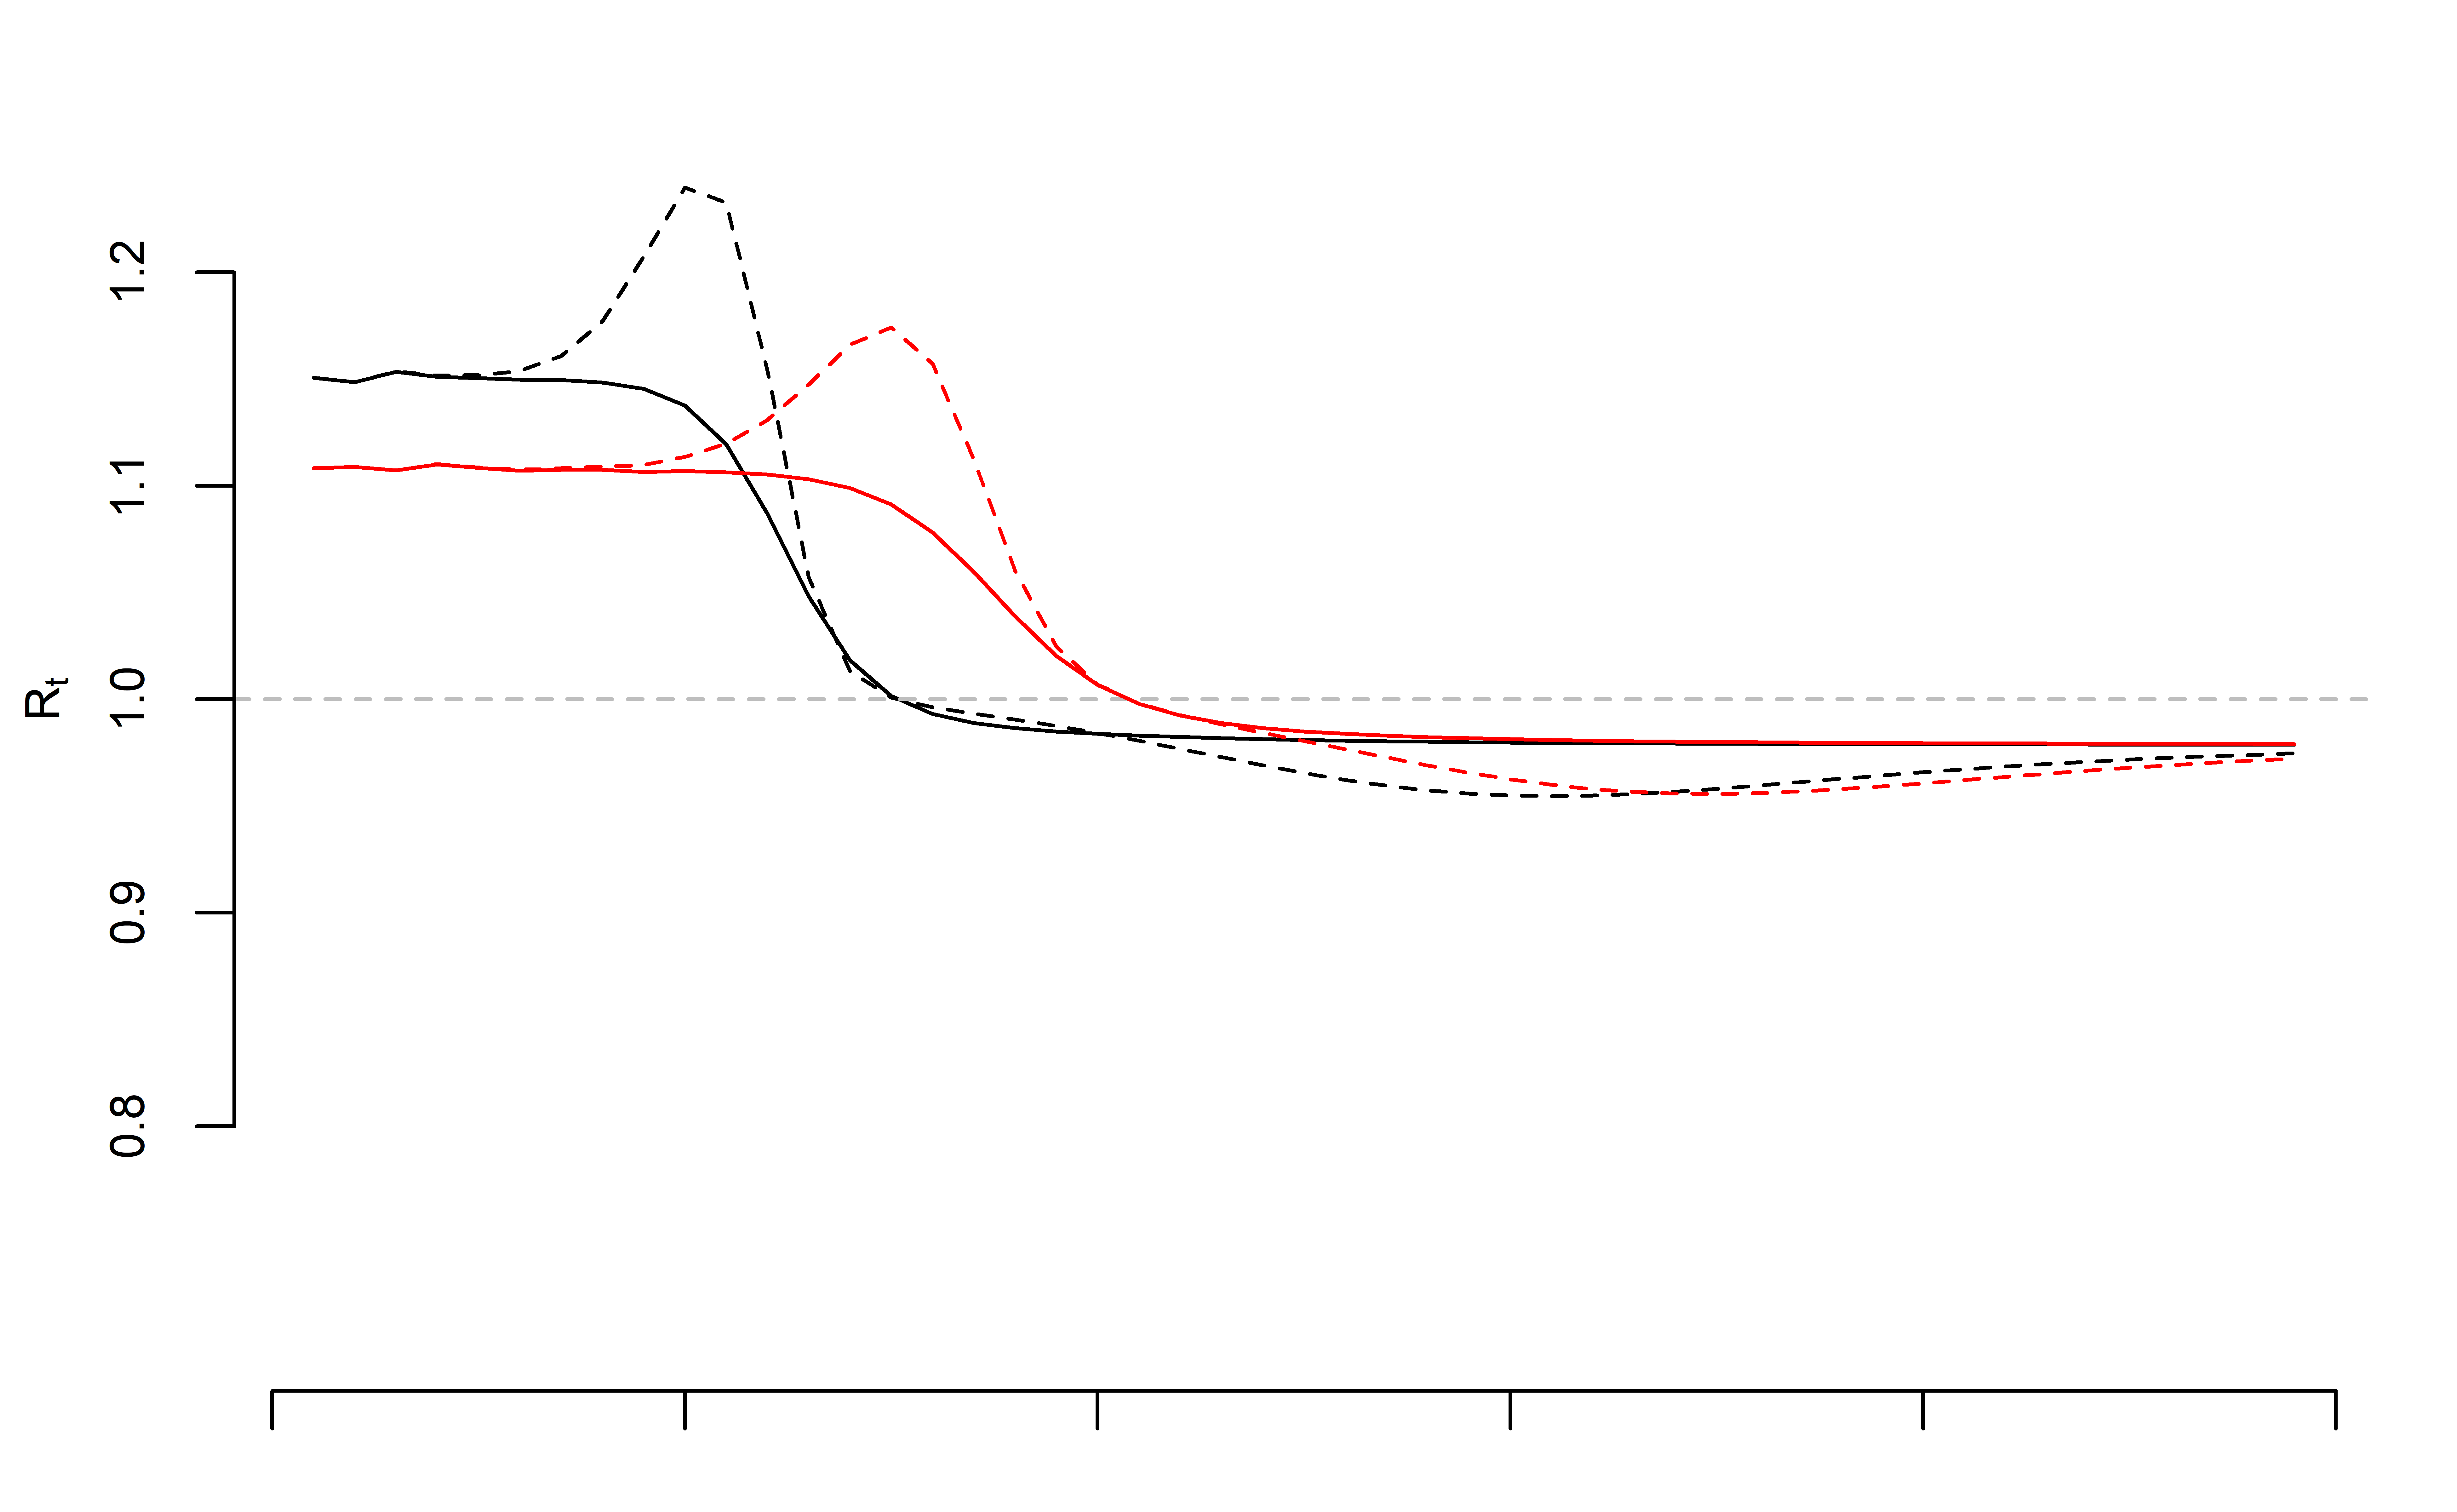
\includegraphics[width=.9\linewidth]{../methods/figs/sir_rt_comparison.png}
  \caption{Effective reproduction rate estimators}
  \label{fig:eff}
\end{subfigure}
\caption{Left: fraction infected in two SIR models with $\beta = 1.4$ and $0.9$ respectively and $\gamma = 0.2$ with same initial conditions. Right: comparison of $\hat R_t$ across time with $FN = 0.2$, $FP = 0.01$, and $M = 4$.}
\label{fig:comparison}
\end{figure}

\subsection{Estimation of Data Quality}
\label{section:est_dq}

In prior sections, we have discussed the impact of selection bias and measurement error on a range of outcomes of interest in COVID-19 research.  Here, we try and address the empirical question of how to estimate the data quality $E_{\I} \left[ \rho_{I,Y} \right]$ in the current context.
In \cite{Meng2018}, estimation of the data quality relied on observing the true outcome.  In election data, for example, we observe the vote totals after the fact and can use this as ground truth.  We are not so lucky in the current crisis.  Here, we propose a simple procedure that uses survey samples as noisy but unbiased estimates of the true prevalence. Our goal is less inferential and more to provide a sensitivity analysis that can aid in understanding the amount of information in observational COVID case-count data.

On April 23rd, Andrew Cuomo announced results from a study in New York state.  It found 13.9\% of 3,000 people tested across the state had signs of the virus.  The study did not report sensitivity and specificity; therefore, we take reported measures from the Santa Clara study~\citep{Bendavid2020} \footnote{We recognize the debate regarding its conclusions.  Here we are only using this study for its information regarding measurement error rates.}.  The reported specificity is $82.8\%$ (95\% CI: 76.0-88.4\%) and sensitivity is $99.5\%$ (95\% CI: 99.2-99.7\%).  This corresponds to a false negative rate of $17.2\%$ (11.6-24.0\%) and false positive rate of $0.5\%$ (0.3 - 0.8\%).  Correcting for these rates we have an estimated prevalence of $15.9\%$ with a range of 14.8\% to 17.0\% using the ranges of the false positive and negative rates.

Figure~\ref{fig:ny-covid-test} plots the number of new total and positive tests per day.  Figure~\ref{fig:ny-covid} plots the fraction of tests that were positiver per day.  In both cases, we applied an exponential smoothing to the reported values because the spiky pattern is likely due to testing backlogs.  Given the report was on the 23rd, we suppose for simplicity that the study was run several days prior on the 20th of April. On the 20th, there were $19,654$ tests performed and $617,555$ tests had been performed up to to and including the 19th. The population of New York state is $19,378,102$.   Subtracting off the number of individuals who had already been tested yields a sampling fraction of $f = 0.001$ on the 20th.  The smoothed prevalence estimate on the 20th is 28.3\%.  Adjusting for measurement error yields an estimate of $32.5\%$.

Here, we assume the New York survey is a simple random sample from the state's population. We recognize that the survey is not such a sample, but techniques like poststratification and raking can be applied to calibrate estimates. Then the error is $16.6$\%.  Using~\eqref{eq:error}, we can use the error to construct an estimate of the relative sampling rate:
\[
\rho D_M = \sqrt{\frac{f}{1-f}} \frac{\text{0.166}}{\sigma_Y} = 1.43 \times 10^{-2} \Rightarrow \Delta = 1.06 \times 10^{-3} \Rightarrow M = 2.29.
\]
The range for the CIs is (2.05, 2.54).  We can also perform sensitivity as a function of the false negative and positive rates.  Under these measurement error ranges, we saw that the impact on the effective reproductive rate estimator was much smaller.  However, for $FP = 0.05$ and $FN = 0.005$ we have $M = 4.31$.  While nothing above is definitive, it points to the interplay of selection bias and measurement error.  This calculation gives us simple tools to understand how sensitivity and specificity impact our estimators and therefore how much we should trust conclusions based on these assumptions.  Under the Santa Clara study estimates of these quantities, while we expect impact, the bias is much smaller than under other estimates.

\begin{figure}
\centering
\begin{subfigure}{.5\textwidth}
  \centering
  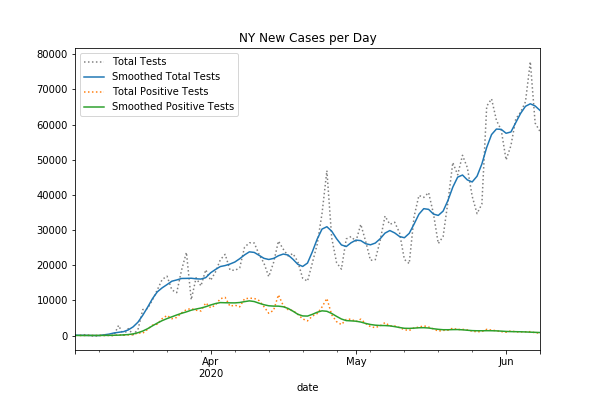
\includegraphics[width=.9\linewidth]{../methods/figs/NY_casecount.png}
  \caption{NY new cases per day}
  \label{fig:ny-covid-test}
\end{subfigure}%
\begin{subfigure}{.5\textwidth}
  \centering
  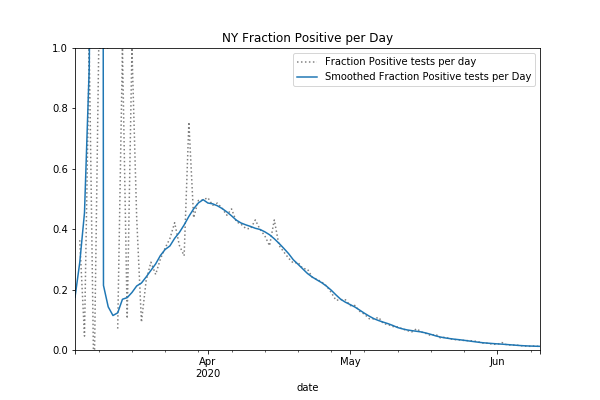
\includegraphics[width=.9\linewidth]{../methods/figs/NY_fracpos.png}
  \caption{NY fraction of new tests positive per day}
  \label{fig:ny-covid-frac}
\end{subfigure}
\caption{New York COVID-19 reported data }
\label{fig:ny-covid}
\end{figure}

\section{Stratified sampling: improving precision in low-prevalence environments}

This article argues why random sampling is a powerful tool and the limitations of data obtained through a self-selection process.  As COVID-19 survey studies become more readily accessible, we encourage researchers to focus on building representative samples.  One difficulty in the current crisis is the low prevalence relative to the population size in certain geographies.  Take the recent Santa Clara study, for example, that estimated less than 2\% prevalence in the area.  The key issue with low prevalence is that if the test's specificity is not lower than the prevalence, then the observed data is consistent with zero recovered individuals.

In such settings, simple random sampling is doomed to fail; however, there are potential solutions.  In particular, one can stratify the population into risk categories (based on population density, occupation, age, and other important factors) and perform Neyman allocation~\citep{Cochran77}.  That is, sample individuals at random in strata $h$ with size proportional to $P_h \sqrt{\bar Y_h \times (1-\bar Y_h)}$ where $P_h$ is the strata frequency in the population and $\bar Y_h$ the prevalence in the strata. Of course, $P_h$ and $\bar Y_h$ are not known a priori; however, if decent estimates can be obtained, we can see huge benefits in settings where the prevalence varies widely by strata. One could go attempt to go further and incorporate contact network information.  However, such data is difficult to obtain in practice.  Indeed, geographic location, occupation, age and basic demographic information are much easier to obtain and are a good proxy for the latent network connectivity.

% \section{Decision-making: data versus information.}

% Having read through the above technical discussions, one may come to the incorrect conclusion that because we are concerned about implicit biases in observational data, we must wait for better data sources in order to act~\citep{Ioannidis2020}.  This conclusion confuses data and information.  Lack of high quality data means we should be skeptical regarding conclusions drawn from these data sources alone.  There are whole fields dedicated to careful analysis in such settings (e.g., causal inference from observational studies).  Being a data skeptic, does not mean one must wait for high quality data to act, especially in high risk scenarios.  One aims to have high quality information.  Yet, in the current crisis, we have just that.  Indeed, epidemiologists and public health officials have a strong understanding of the basic facts of pandemics and disease spread.  Social distancing, contact tracing and mass testing are all important.  Individuals and populations with low quality data and only basic information will make decisions that respect inherent risks in unknown unknowns. Of course, there are trade-offs and long-term stay-at-home orders will have negative economic consequences.  A full discussion of these topics is beyond the scope of the current article; we merely bring up the matter because we are well aware that discussions of data quality can sometimes be misinterpreted as claims that we do not have the requisite information to act immediately and decisively.  This is simply not the case.

\section{Discussion}
\label{section:discussion}

There is nothing routine about COVID-19, including the corresponding statistical questions.  The goal of this paper was to point out questionable statistical routines.  Indeed, case-count trajectories are being reported daily by governments and broadcast by the media.  The precision in the reported numbers gives the illusion of accuracy when what needs to be understood is the level of uncertainty. Selection bias not only means uncertainty, it also implies analysts feel certain about incorrect conclusions.  We end this paper with a brief discussion of several important topics related to selection bias and measurement error.

\subsection*{Decision-making: data versus information}

Having read through the above technical discussions, one may come to the incorrect conclusion that because we are concerned about implicit biases in observational data, we must wait for better data sources in order to act~\citep{Ioannidis2020}.  This conclusion confuses data and information.  Lack of high quality data means we should be skeptical regarding conclusions drawn from these data sources alone.  Being skeptical of observed data does not imply governments and communities should wait for high quality data to act; this is especially true in the current high risk scenario.  Instead, we should aim to have high quality information.  Yet in the current crisis we have just that.  Indeed, epidemiologists and public health officials have a strong understanding of the basic facts of pandemics and disease spread.  Social distancing, contact tracing and mass testing are all important.  Individuals and communities with low quality data and only basic information will hopefully make decisions that respect inherent risks to their well being as well as the high degree of uncertainty in the observed data. Of course, there are trade-offs and long-term stay-at-home orders will have negative economic consequences.  A full discussion of these topics is beyond the scope of the current article.

\subsection*{High quality information on prevalence.}

Governments are pushing for increased testing capacity and robust contact tracing.  Contact tracing is incredibly useful for identifying carriers early and preventing spread of the disease.  We would argue that, after the current wave, understanding prevalence is also key.  We know that the probability of an outbreak is a function of current prevalence and network connectivity.  Epidemic critical thresholds have been derived for many infectious disease models~\cite{Pastor2001,Newman2002,Parshani2010}.  Knowing prevalence will help governments determine long-term community-level risk and allow for more targeted interventions -- shutting down only certain locations when necessary.

\subsection*{Data quantity versus quality}

Governments implicitly argue that increased testing capacity will perform the above task.  Without complete compliance, however, our understanding of future outbreaks may be plagued by self-selection bias, compounded by changing sensitivity and specificity rates. Random testing removes these effect modifiers, giving governments more information to fight the disease.  This is not to say random testing should replace current testing practices; only that the random testing should supplement and will provide valuable additional information even with moderate sample sizes.

% Not only that, in current crisis data quality is often tied to data quantity due to rationing system.  Increasing testing under test rationing lowers correlation.  There is a lot of hidden information in the selection indicator $I_j$.  Indeed, individuals must first seek testing and then call their primary health care provider must decide whether they met thresholds for testing.  Our analysis shows the limitations and caveats that come from analysis of this data in terms of estimation of prevalence, rates of change, and cross-country comparisons.  We show how one can build simple sensitivity analyses to understand the potential bias in case-count data using surveys that will become more prevalent in the next few months.

\subsection*{Model-based solutions.}

One alternative approach to what is presented in this article is a model-based extension of SIR models to try and capture both selection bias and measurement error; however, without strong assumptions on the selection mechanism, the estimates are often not nonparametrically identifiable.  When an issue ``cannot be resolved nonparametrically then it is usually dangerous to resolve it parametrically'' ~\cite[pp. 96]{CoxHink74}. In the absence of randomized experiments, the best route forward using any approach is the use of detailed sensitivity analyses and humility in conclusions drawn from such data sources.

\bibliographystyle{plainnat}
\bibliography{covid-refs}

\appendix

\section{Imperfect testing: derivation}
\label{app:imperfect}
We considered the mean estimator
$$
\bar y_n^\star = \frac{\sum_{j=1}^N Y_j^\star I_j}{\sum_{j=1}^N I_j} = \frac{\sum_{i=1}^N  I_j Y_j^\star }{\sum_{j=1}^N  I_j } = \frac{\sum_{i=1}^N  I_j \left[ Y_j (1-P_j) + (1-Y_j) P_j \right]}{\sum_{j=1}^N  I_j }
$$
For any set of numbers $\{ A_1, \ldots, A_N \}$ we can view it as the support of a random variable $A_J$ induced by the random index $J$ defined on $\{1,\ldots, N\}$.  When $J$ is uniformly distributed $E_J (A_J) = \sum_{j=1}^N A_j / N \equiv \bar A_N$. Then
$$
\begin{aligned}
\bar y_n^\star  - \bar Y_N &= \frac{E_J \left[ I_J \left[ Y_J (1-P_J) + (1-Y_J) P_J \right] \right]}{E_J [ I_J ] } - E_J[Y_J] \\
&= \frac{E_J \left[ I_J P_J (1-2Y_J) \right]}{E_J [ I_J ] } + \left( \frac{E_J [I_J Y_J]}{E_J [ I_J ] } - \frac{E_J[Y_J] E_J[I_J]}{E_J[I_J]} \right) \\
\end{aligned}
$$
The term in parentheses can be re-written as
$$
\begin{aligned}
\frac{E_J [I_J Y_J]- E_J[Y_J] E_J[I_J]}{E_J[I_J]} &=  \frac{E_J [I_J Y_J]- E_J[Y_J] E_J[I_J]}{\sqrt{V_J(I_J) V_J(Y_J)}} \frac{\sqrt{V_J(I_J)}}{E_J[I_J]} \times \sqrt{V_J(Y_J)} \\
&= \rho_{I,Y} \times \sqrt{\frac{(1-f)}{f}} \times \sigma_Y
\end{aligned}
$$
which agrees with Meng's (2019) decomposition. For the other term, first we define $Z_j := 1 - 2 Y_j $. Then $Z_j = 1$ if $Y_j = 0$ and $Z_j = -1$ if $Y_j = 1$. Then the term can be re-written as
$$
\begin{aligned}
\frac{E_J \left[ I_J P_J (1-2Y_J) \right]}{E_J [ I_J ] } &= \left( \frac{E_J \left[ I_J P_J Z_J \right]}{E_J [ I_J ] } -  \frac{E_J \left[ P_J Z_J \right] E_J[ I_J]}{E_J [ I_J ] } \right) +  \frac{E_J \left[ P_J Z_J \right] E_J[ I_J]}{E_J [ I_J ] } \\
\end{aligned}
$$
The term in parentheses can be re-expressed using the previous technique as:
$$
\rho_{I, PZ} \times \sqrt{\frac{1-f}{f}} \times \sigma_{PZ}
$$
where now the ``data defect'' and ``problem difficulty'' are with respect to $PZ$ rather than $Y$. The final term is equal to
$$
\begin{aligned}
E_J [P_J Z_J ] &= E_J [ E_J [ P_J Z_J \mid Y_J ] ] \\
&= \pr (P = 1 \mid Y = 0) (1-\bar Y) - \pr(P=1 \mid Y = 1) \bar Y \\
&= FP - (FP + FN) \cdot \bar Y
\end{aligned}
$$
Combining these yields:
$$
\bar y_n^\star - \bar Y = \sqrt{\frac{1-f}{f}} \left[\rho_{I,Y} \sigma_Y + \rho_{I, PZ} \sigma_{PZ} + \sqrt{\frac{f}{1-f}} \left( FP - (FP+FN) \bar Y \right) \right]
$$
For the binary outcome $Y$, we have $\sigma_Y = \sqrt{\bar Y (1-\bar Y)}$. Moreover,
$$
\begin{aligned}
V_J(P_J Z_J) &= E_J[(P_J Z_J)^2] - E[P] E[Z] \\
&= E[P] - E[P] (1 - 2 \bar Y) = 2 \bar Y E_J [ P_J ] \\
&= 2 \bar Y \left( FP (1-\bar Y) + FN \bar Y \right) \\
\Rightarrow \sigma_{PZ} &= \sqrt{ 2 \bar Y \left( FP (1-\bar Y) + FN \cdot  \bar Y \right) }
\end{aligned}
$$
Then the formula for the error is given by:
$$
\sqrt{\frac{1-f}{f}} \left[\rho_{I,Y} \sqrt{\bar Y (1-\bar Y)} + \rho_{I, PZ} \sqrt{ 2 \bar Y \left( FP (1-\bar Y) + FN \cdot \bar Y \right )} + \sqrt{\frac{f}{1-f}} \left( FP - (FP+FN) \bar Y \right) \right]
$$

\subsection{Estimate of observed data quality}

By definition, we have
$$
\begin{aligned}
\rho_{I,PZ} &= \frac{C(I, PZ)}{\sqrt{V(PZ) V(I)}} \\
&= \frac{C(I, PZ)}{\sqrt{V(Y) V(I)}} \sqrt{\frac{V(Y)}{V(PZ)}} \\
&= \rho_{I,Y} \frac{C(I,PZ)}{C(I,Y)} \sqrt{ \frac{(1-\bar Y)}{2 ( FP (1-\bar Y) + FN \cdot \bar Y)} }
\end{aligned}
$$

$$
\begin{aligned}
C(I, PZ) &= E[ I P Z ] - E[I] E[PZ] \\
&=  [FP f_0 - (FP f_0 + FN f_1) \bar Y] - f [ FP - (FP+FN) \bar Y ] \\
&=  - FP \Delta \bar Y + FP \bar Y^2 \Delta - FN \bar Y^2 \Delta \\
&=  - \Delta \bar Y (FP \cdot (1-\bar Y) + FN \cdot \bar Y) \\
\end{aligned}
$$
where $f = f_1 \bar Y + f_0 (1-\bar Y)$ so $f_0 - f = -\Delta \bar Y$ and $f_1 - f = \Delta (1-\bar Y)$.
$$
\begin{aligned}
C(I, Y) &= E[ I Y ] - f \bar Y \\
&=  f_1 \bar Y + f_0 (1-\bar Y) - f \bar Y \\
&=  f_0 (1-\bar Y) + \Delta (1-\bar Y) \bar Y \\
&= (1-\bar Y) (f_0 + \Delta \bar Y)
\end{aligned}
$$
Combining yields
$$
\begin{aligned}
\rho_{I,PZ} &= \rho_{I,Y} \times \frac{- \Delta \bar Y (FP \cdot (1-\bar Y) + FN \cdot \bar Y) }{(1-\bar Y) (f_0 + \Delta \bar Y)} \times \sqrt{ \frac{(1-\bar Y)}{2 ( FP (1-\bar Y) + FN \cdot \bar Y)} } \\
&= - \rho_{I, Y} \times \Delta \times \sqrt{\frac{\bar Y}{1-\bar Y}} \frac{\sqrt{FP(1-\bar Y) + FN \cdot \bar Y}}{f_0 (1-\bar Y) + f_1 \bar Y} \times \sqrt{\frac{\bar Y}{2}}
\end{aligned}
$$
We can then re-write $\rho_{I,Y} \sigma_Y + \rho_{I,PZ} \sigma_{PZ}$ as
$$
\rho_{I,Y} \sigma_Y \left( 1 - \Delta \times \frac{\bar Y}{1-\bar Y} \times \frac{FP(1-\bar Y) + FN \cdot \bar Y}{f_0 (1-\bar Y) + f_1 \bar Y} \right)
$$
Suppose $f_1 = M \cdot f_0$.  Then $\Delta = f_1 - f_0 = f_0 (M-1)$ and $f_0 (1-\bar Y) + f_1 \bar Y = f_0 ( (1-\bar Y) + M \bar Y )$ and we can re-write above as
$$
\rho_{I,Y} \sigma_Y \left( 1 - (M-1) \times \frac{\bar Y}{1-\bar Y} \times \frac{FP(1-\bar Y) + FN \cdot \bar Y}{(1-\bar Y) + M \bar Y} \right).
$$

\subsection{Ratio estimator}
\label{app:ratio}

Let ${\bf u} = (u_{t-1},u_t) \in \mathbb{R}^2$ and $g({\bf u}) = \frac{u_t}{u_{t-1}}$, i.e., a differentiable function $g:\mathbb{R}^2 \to \mathbb{R}$. Centering a Taylor series expansion of second-order around coordinates $(U_2, U_1) \in \mathbb{R}^2$ yields
$$
\begin{aligned}
g({\bf u}) =& g(U_{t-1}, U_t) - \frac{U_t}{U_{t-1}^2} (u_{t-1} - U_{t-1}) + \frac{1}{U_{t-1}} (u_t - U_t) \\
&+ \frac{1}{2} \left[ \frac{2 U_t}{U_{t-1}^3} (u_{t-1} - U_{t-1})^2 + 0 \times (u_t - U_t)^2 - 2 \times (u_{t-1} - U_{t-1}) (u_t - U_t) \frac{1}{U_t^2} \right]
\end{aligned}
$$
Plugging in $(\bar y_{t-1}, \bar y_t)$ for $(u_{t-1}, u_t)$ and $(\bar Y_{t-1}, \bar Y_t)$ for $(U_{t-1}, U_t)$ yields the $\frac{\bar y_t}{\bar y_{t-1}} - \frac{\bar Y_t}{\bar Y_{t-1}} $ is equal to
$$
\begin{aligned}
=&
- \frac{\bar Y_t}{\bar Y_{t-1}^2} (\bar y_{t-1} - \bar Y_{t-1}) + \frac{1}{\bar Y_{t-1}} (\bar y_t - \bar Y_t) \\
&+ \frac{\bar Y_t}{\bar Y_{t-1}^3} (\bar y_{t-1} - \bar Y_{t-1})^2 -  (\bar y_{t-1} - \bar Y_{t-1}) (\bar y_t - \bar Y_t) \frac{1}{\bar Y_{t-1}^2} \\
&= \frac{\bar Y_t}{\bar Y_{t-1}} \bigg[  \rho_{I_t,Y_t} \sqrt{\frac{1-f_t}{f_t}} CV (Y_t)  -\rho_{I_{t-1},Y_{t-1}} \sqrt{\frac{1-f_{t-1}}{f_{t-1}}} CV (Y_{t-1}) \\
&+ \rho^2_{I_{t-1},Y_{t-1}} \frac{1-f_{t-1}}{f_{t-1}} CV^2 (Y_{t-1}) -  \rho_{I_{t-1},Y_{t-1}} \sqrt{\frac{1-f_{t-1}}{f_{t-1}}} CV (Y_{t-1}) \times
\rho_{I_t,Y_t} \sqrt{\frac{1-f_t}{f_t}} CV (Y_t)   \bigg] \\
&= \frac{\bar Y_t}{\bar Y_{t-1}} \bigg[ \rho_{I_t,Y_t} \sqrt{\frac{1-f_t}{f_t}} CV (Y_t)  -\rho_{I_{t-1},Y_{t-1}} \sqrt{\frac{1-f_{t-1}}{f_{t-1}}} CV (Y_{t-1}) \bigg] \left[ 1 - \rho_{I_{t-1},Y_{t-1}} \sqrt{\frac{1-f_{t-1}}{f_{t-1}}} CV (Y_{t-1}) \right]
\end{aligned}
$$
where the second equality is obtained by plugging in the statistical decomposition of the error for both time points and the coefficient of variation being defined as $CV(Y) := \sigma_Y/\mu_Y$.  Under measurement error, the extra terms $D_{2}$ and $D_1$ can be inserted in the correct locations.

\subsection{Estimation of effective reproduction number}

Let
$$
\delta_t := \bigg[ \rho_{I_t,K_t} D_{M_t} \sqrt{\frac{1-f_t}{f_t}} CV (K_t)  -\rho_{I_{t-1},K_{t-1}} D_{M_{t-1}} \sqrt{\frac{1-f_t}{f_t}} CV (K_{t-1}) \bigg].
$$
Then results from Section~\ref{app:ratio} show that the estimate of the number of new cases on day t is given by
$$
\frac{S_t \cdot \bar y_t}{S_{t-1} \cdot \bar y_{t-1}} =
\frac{K_t}{K_{t-1}} \left( 1 + \delta_t \times \left[ 1 - \rho_{I_{t-1},K_{t-1}} D_{M_{t-1}} \sqrt{\frac{1-f_t}{f_t}} CV (K_{t-1}) \right] \right)
$$
Then setting $e_t = \delta_t \times [1 - \rho_{I_{t-1},K_{t-1}} D_{M_{t-1}} \sqrt{\frac{1-f_t}{f_t}} CV (K_{t-1}) ]$, we have
$$
\begin{aligned}
\log \left( \frac{S_t \bar y_t}{S_{t-1} \bar y_{t-1}} \right) - \log \left( \frac{K_t}{K_{t-1}} \right) &= \log (1 + e_t) \\
\log \left( \frac{\bar y_t}{\bar y_{t-1}} \right) - \log \left( \frac{K_t}{K_{t-1}} \right) &= 1 + e_t - \log \left( \frac{S_t}{S_{t-1}} \right) \\
1 + \frac{1}{\gamma} \log \left( \frac{\bar y_t}{\bar y_{t-1}} \right) - \left[ 1 + \frac{1}{\gamma} \log \left( \frac{K_t}{K_{t-1}} \right) \right] &= \frac{1}{\gamma} \left[ \log \left( 1 + e_t \right) - \log \left( \frac{S_{t}}{S_{t-1}} \right) \right] \\
\Rightarrow \hat R_t - R_t &= \frac{1}{\gamma} \left[ \log \left( 1 + e_t \right) - \log \left( \frac{S_{t}}{S_{t-1}} \right) \right]
\end{aligned}
$$



\section{Derivation for the effective sample size}
\label{section:effss}

For binary outcomes, we have
\begin{equation} \label{eq:binaryrho}
\rho_{I,Y} = \Delta \sqrt{\frac{\bar Y (1 - \bar Y)}{f (1-f)} }
\end{equation}
where $\Delta = P_J (I_J = 1 \mid Y_J = 1) - P(I_J = 1 \mid Y_J = 0) = f_1 - f_0$.  Suppose that $M = f_1/f_0$; then
$f_0 = f / (\bar Y \cdot (M-1) + 1)$.  For $\bar Y = 0.091$, $M = 2$ and $f = 0.026$ we have $f_0 = 0.024$ and $f_1 = 0.048$ which implies $\Delta = 0.024$.
Then $\rho_{I,Y} = 0.043$.  Then $E_{\I} [ \rho_{I,Y}^2 ] \leq (E_{\I} [\rho_{I,Y} ]^2 = 0.0019$.  Then
$$
n_{eff} \leq \frac{f}{1-f} \frac{1}{0.0019} = 14.39.
$$
Using this computation, we compute effective sample size under a range of values $\bary$, $M$ with $f = 0.026$ (i.e., current sampling fraction) and $f =1/7$ (sample individuals roughly every 7 days).

\begin{table}[ht]
\centering
\begin{tabular}{rrrrrr}
& \multicolumn{5}{c}{$M$} \\ \cline{2-6}
$\bar y$ & 1.2 & 1.4 & 1.6 & 1.8 & 2 \\
  \hline
0.016 & 1598.00 & 402.00 & 180.00 & 102.00 & 66.00 \\
  0.036 & 731.00 & 185.00 & 84.00 & 48.00 & 31.00 \\
  0.056 & 484.00 & 124.00 & 56.00 & 32.00 & 21.00 \\
  0.076 & 367.00 & 94.00 & 43.00 & 25.00 & 16.00 \\
  0.096 & 299.00 & 78.00 & 36.00 & 21.00 & 14.00 \\
   \hline
\end{tabular}
\end{table}


We also present the same plot under $FP = 0.005$ and $FN = 0.172$ to show the impact of measurement error on effective sample size.

\begin{table}[ht]
\centering
\begin{tabular}{rrrrrr}
  & \multicolumn{5}{c}{$M$} \\ \cline{2-6}
$\bar y$ & 1.2 & 1.4 & 1.6 & 1.8 & 2 \\
  \hline
0.016 & 1154.00 & 290.00 & 130.00 & 73.00 & 47.00 \\
  0.036 & 528.00 & 134.00 & 60.00 & 34.00 & 22.00 \\
  0.056 & 349.00 & 89.00 & 41.00 & 23.00 & 15.00 \\
  0.076 & 265.00 & 68.00 & 31.00 & 18.00 & 12.00 \\
  0.096 & 216.00 & 56.00 & 26.00 & 15.00 & 10.00 \\
   \hline
\end{tabular}
\end{table}


% \section{Quotes}

% I prefer to think of a statistical sensibility rather than statistical thinking. It’s “less than an agenda but more than an attitude.”  It allows for methodological preference while avoiding dogma. Paired with data analytic humility and I think you have proper “data science”


% A test of meaningfulness of a possible model for a data-generating process is whether it can be used directly to simulate data.” (p.104).  In our current setting, this most certainly related to simulation while accounting for measruement error.




\end{document}